In questo capitolo verranno analizzati i risultati prodotti dal simulatore realizzato in questo progetto di tesi.
Durante lo sviluppo di questo simulatore sono stati svolti molti esperimenti relativi al funzionamento dei vari moduli e all'interazione tra flusso e particelle, di seguito,
per ovvie ragioni, mostreremo solo quelli effettuati nello stato più avanzato di sviluppo.
In particolare verranno analizzati i risultati dei vari moduli in maniera separata per poi combinarli in unico risultato sperimentale.
Per assemblare le figure riportate è stato utilizzato Paraview (\ref{paraview}) utilizzando il modulo di RayTracing (\ref{raytracing}).

\section{Mesh}
La mesh è stata generata con Salome (\ref*{salome}) ed è composta da due coni concentrici rivolti verso il basso. Nel cono più esterno passa il fluido e le particelle,
mentre in quello interno il fascio laser. Di seguito una serie di immagini che descrivono al meglio la mesh, notare la disposizione dei vertici e l'aumento di risoluzione in prossimità
dell'uscita dell'ugello.
\begin{figure}[H]\label{dettaglio_ugello}
    \centering
    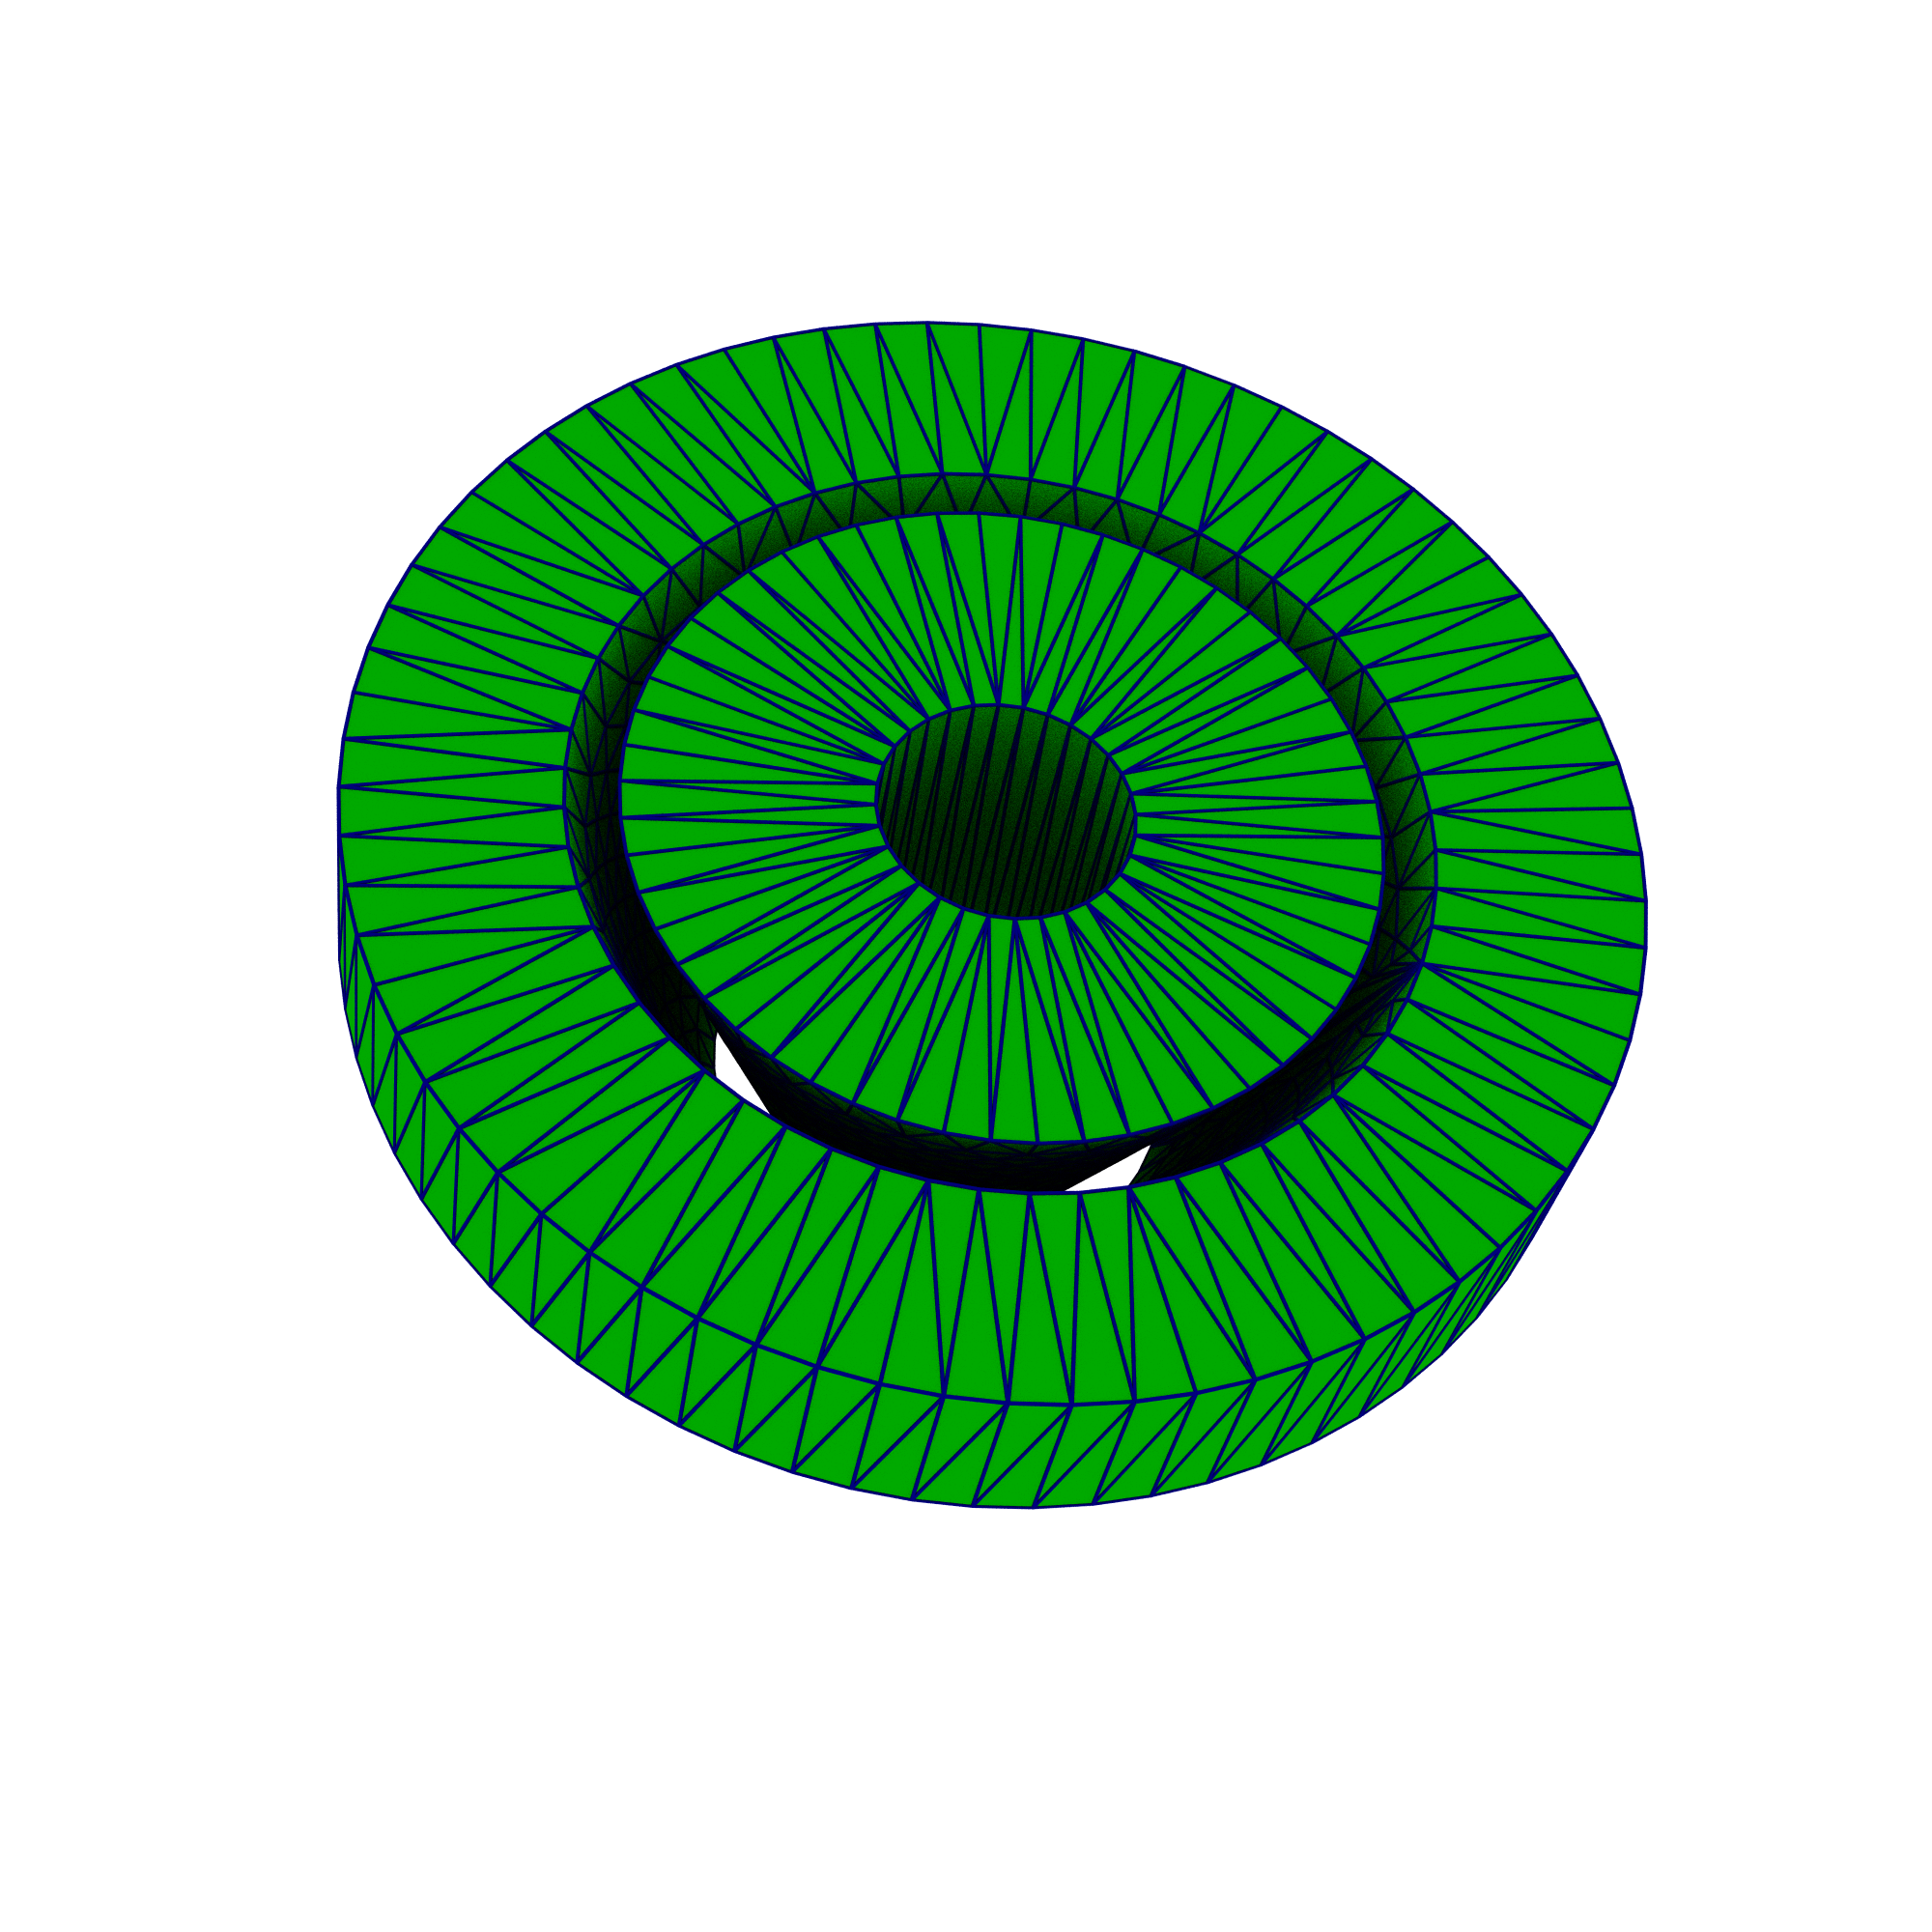
\includegraphics[width=\linewidth]{figure/screenshot_dettaglio_ugello_alto.png}
    \caption{Ugello visto dall'alto.}
\end{figure}
\begin{figure}[H]\label{dettaglio_ugello}
    \centering

    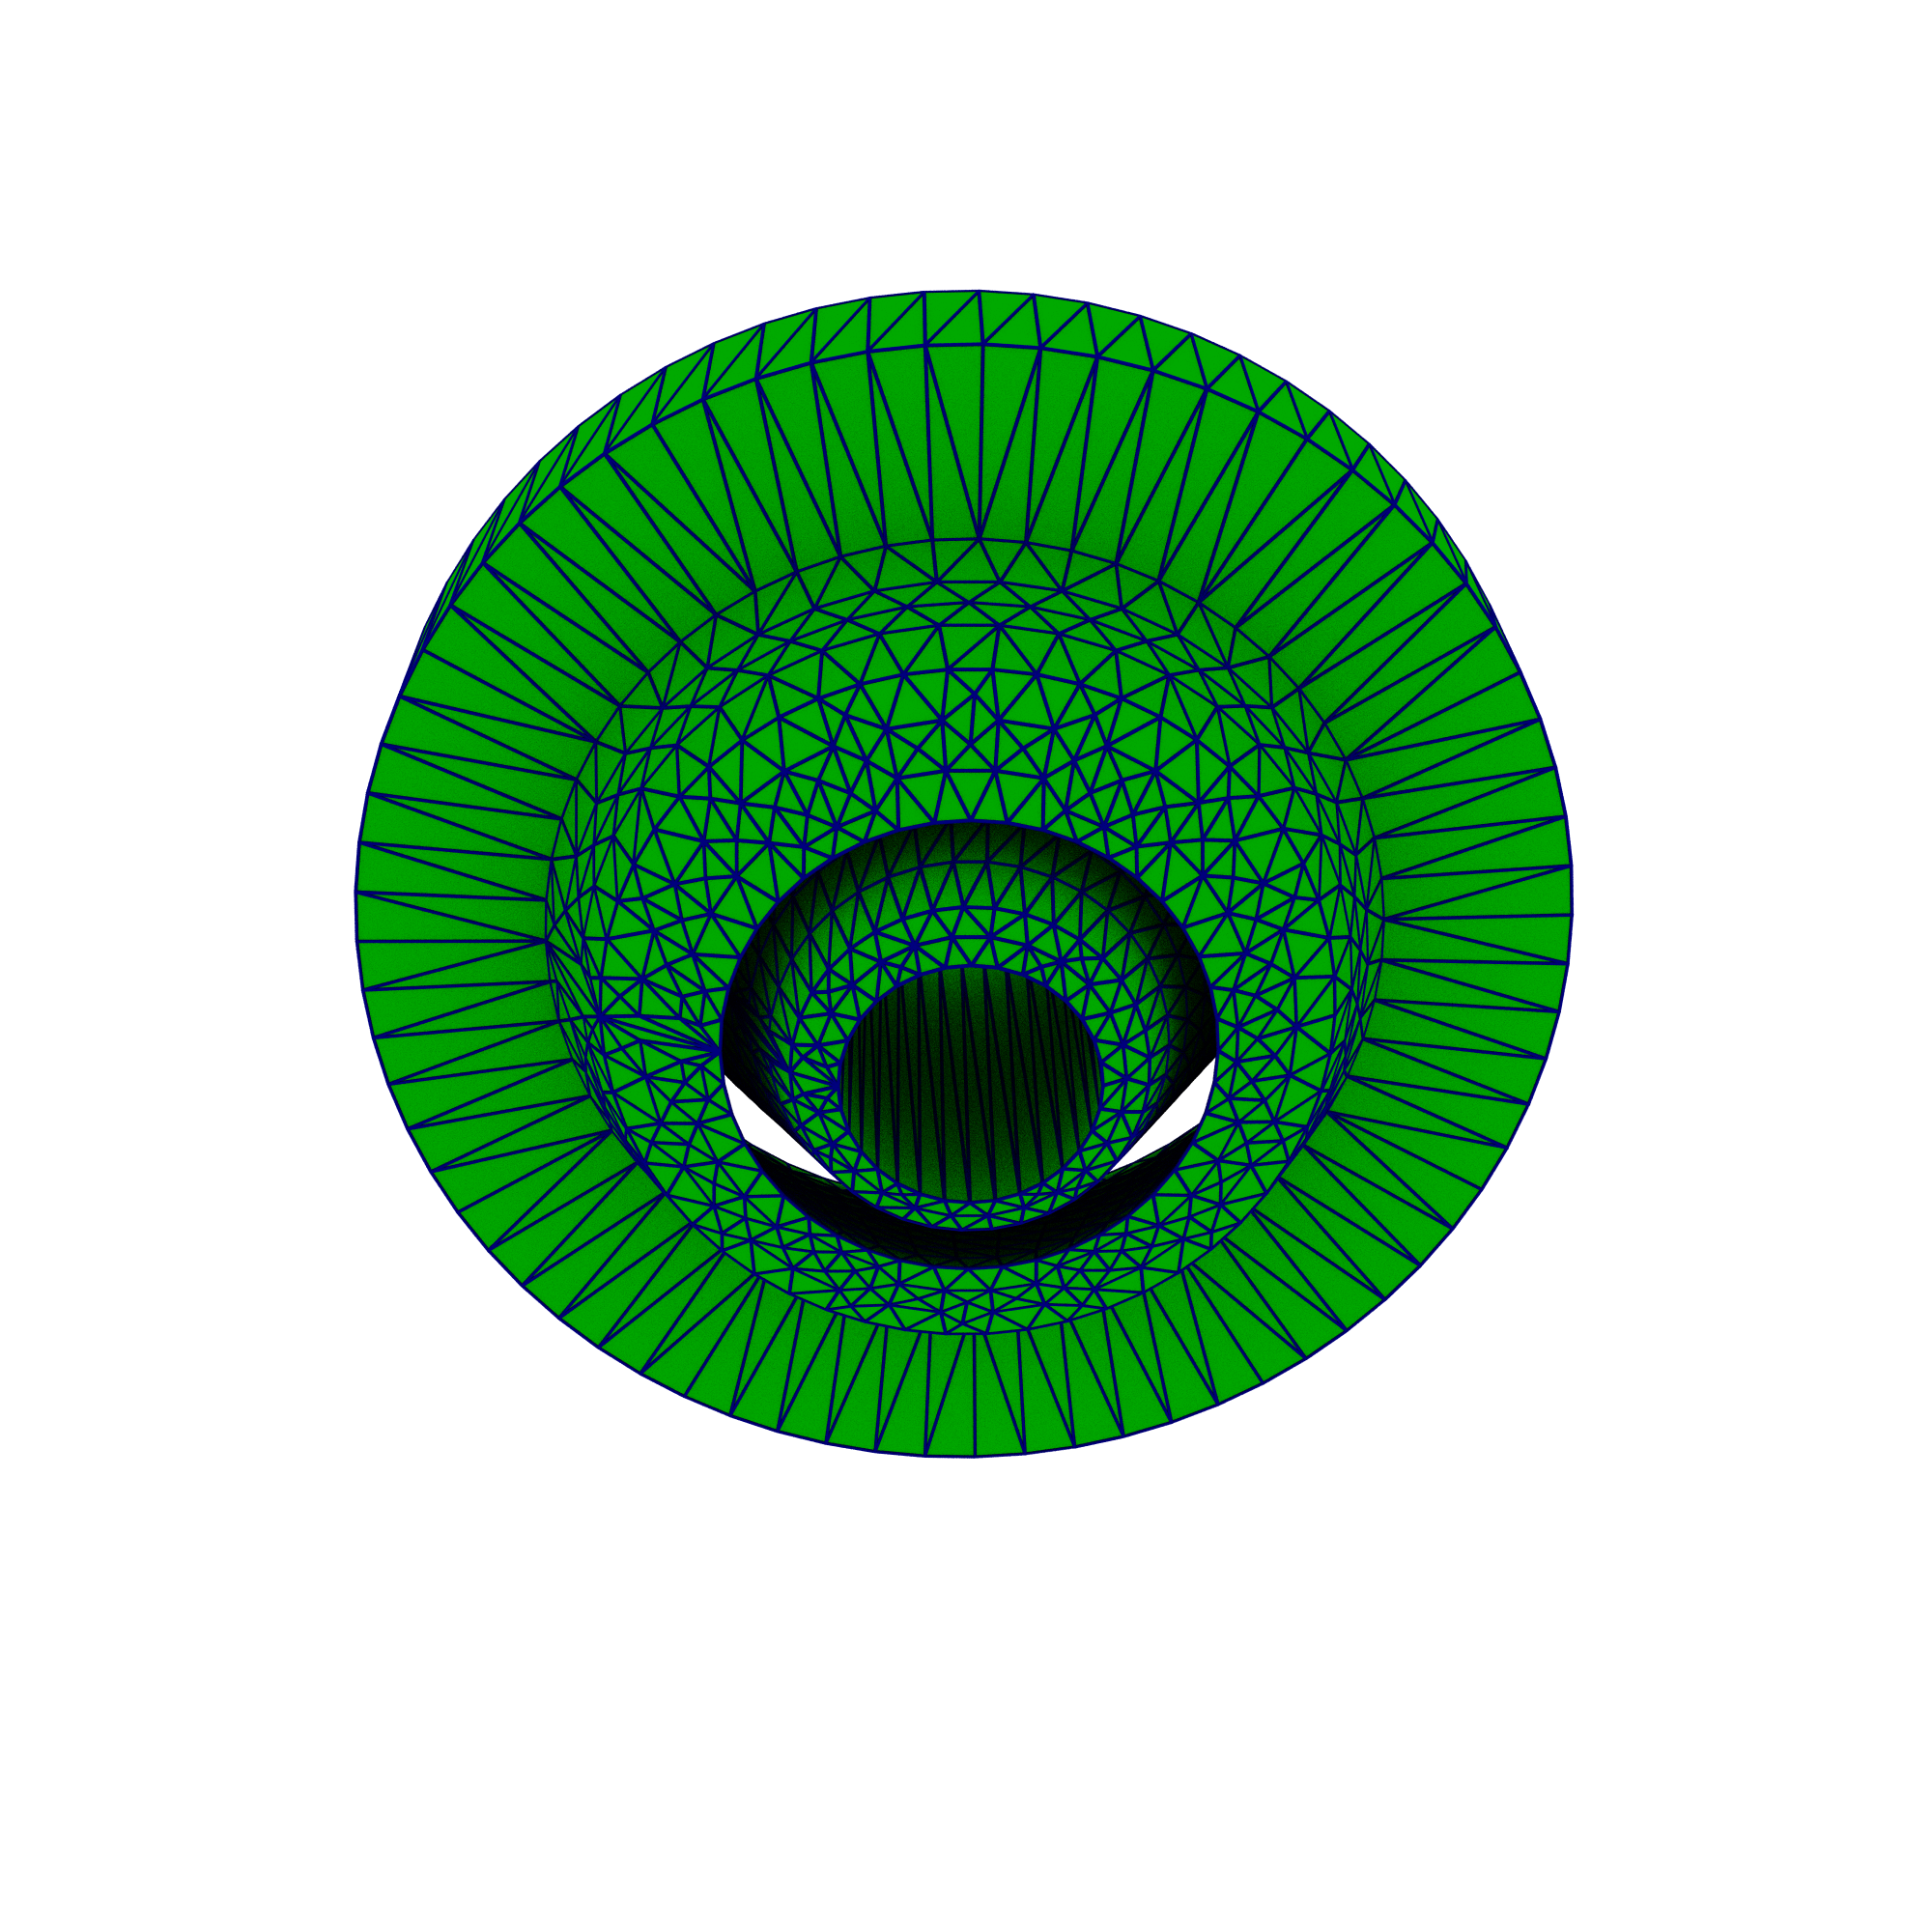
\includegraphics[width=\linewidth]{figure/screenshot_dettaglio_ugello_basso.png}
    \caption{Ugello visto dal basso.}
\end{figure}
\begin{figure}[H]\label{dettaglio_ugello}
    \centering
    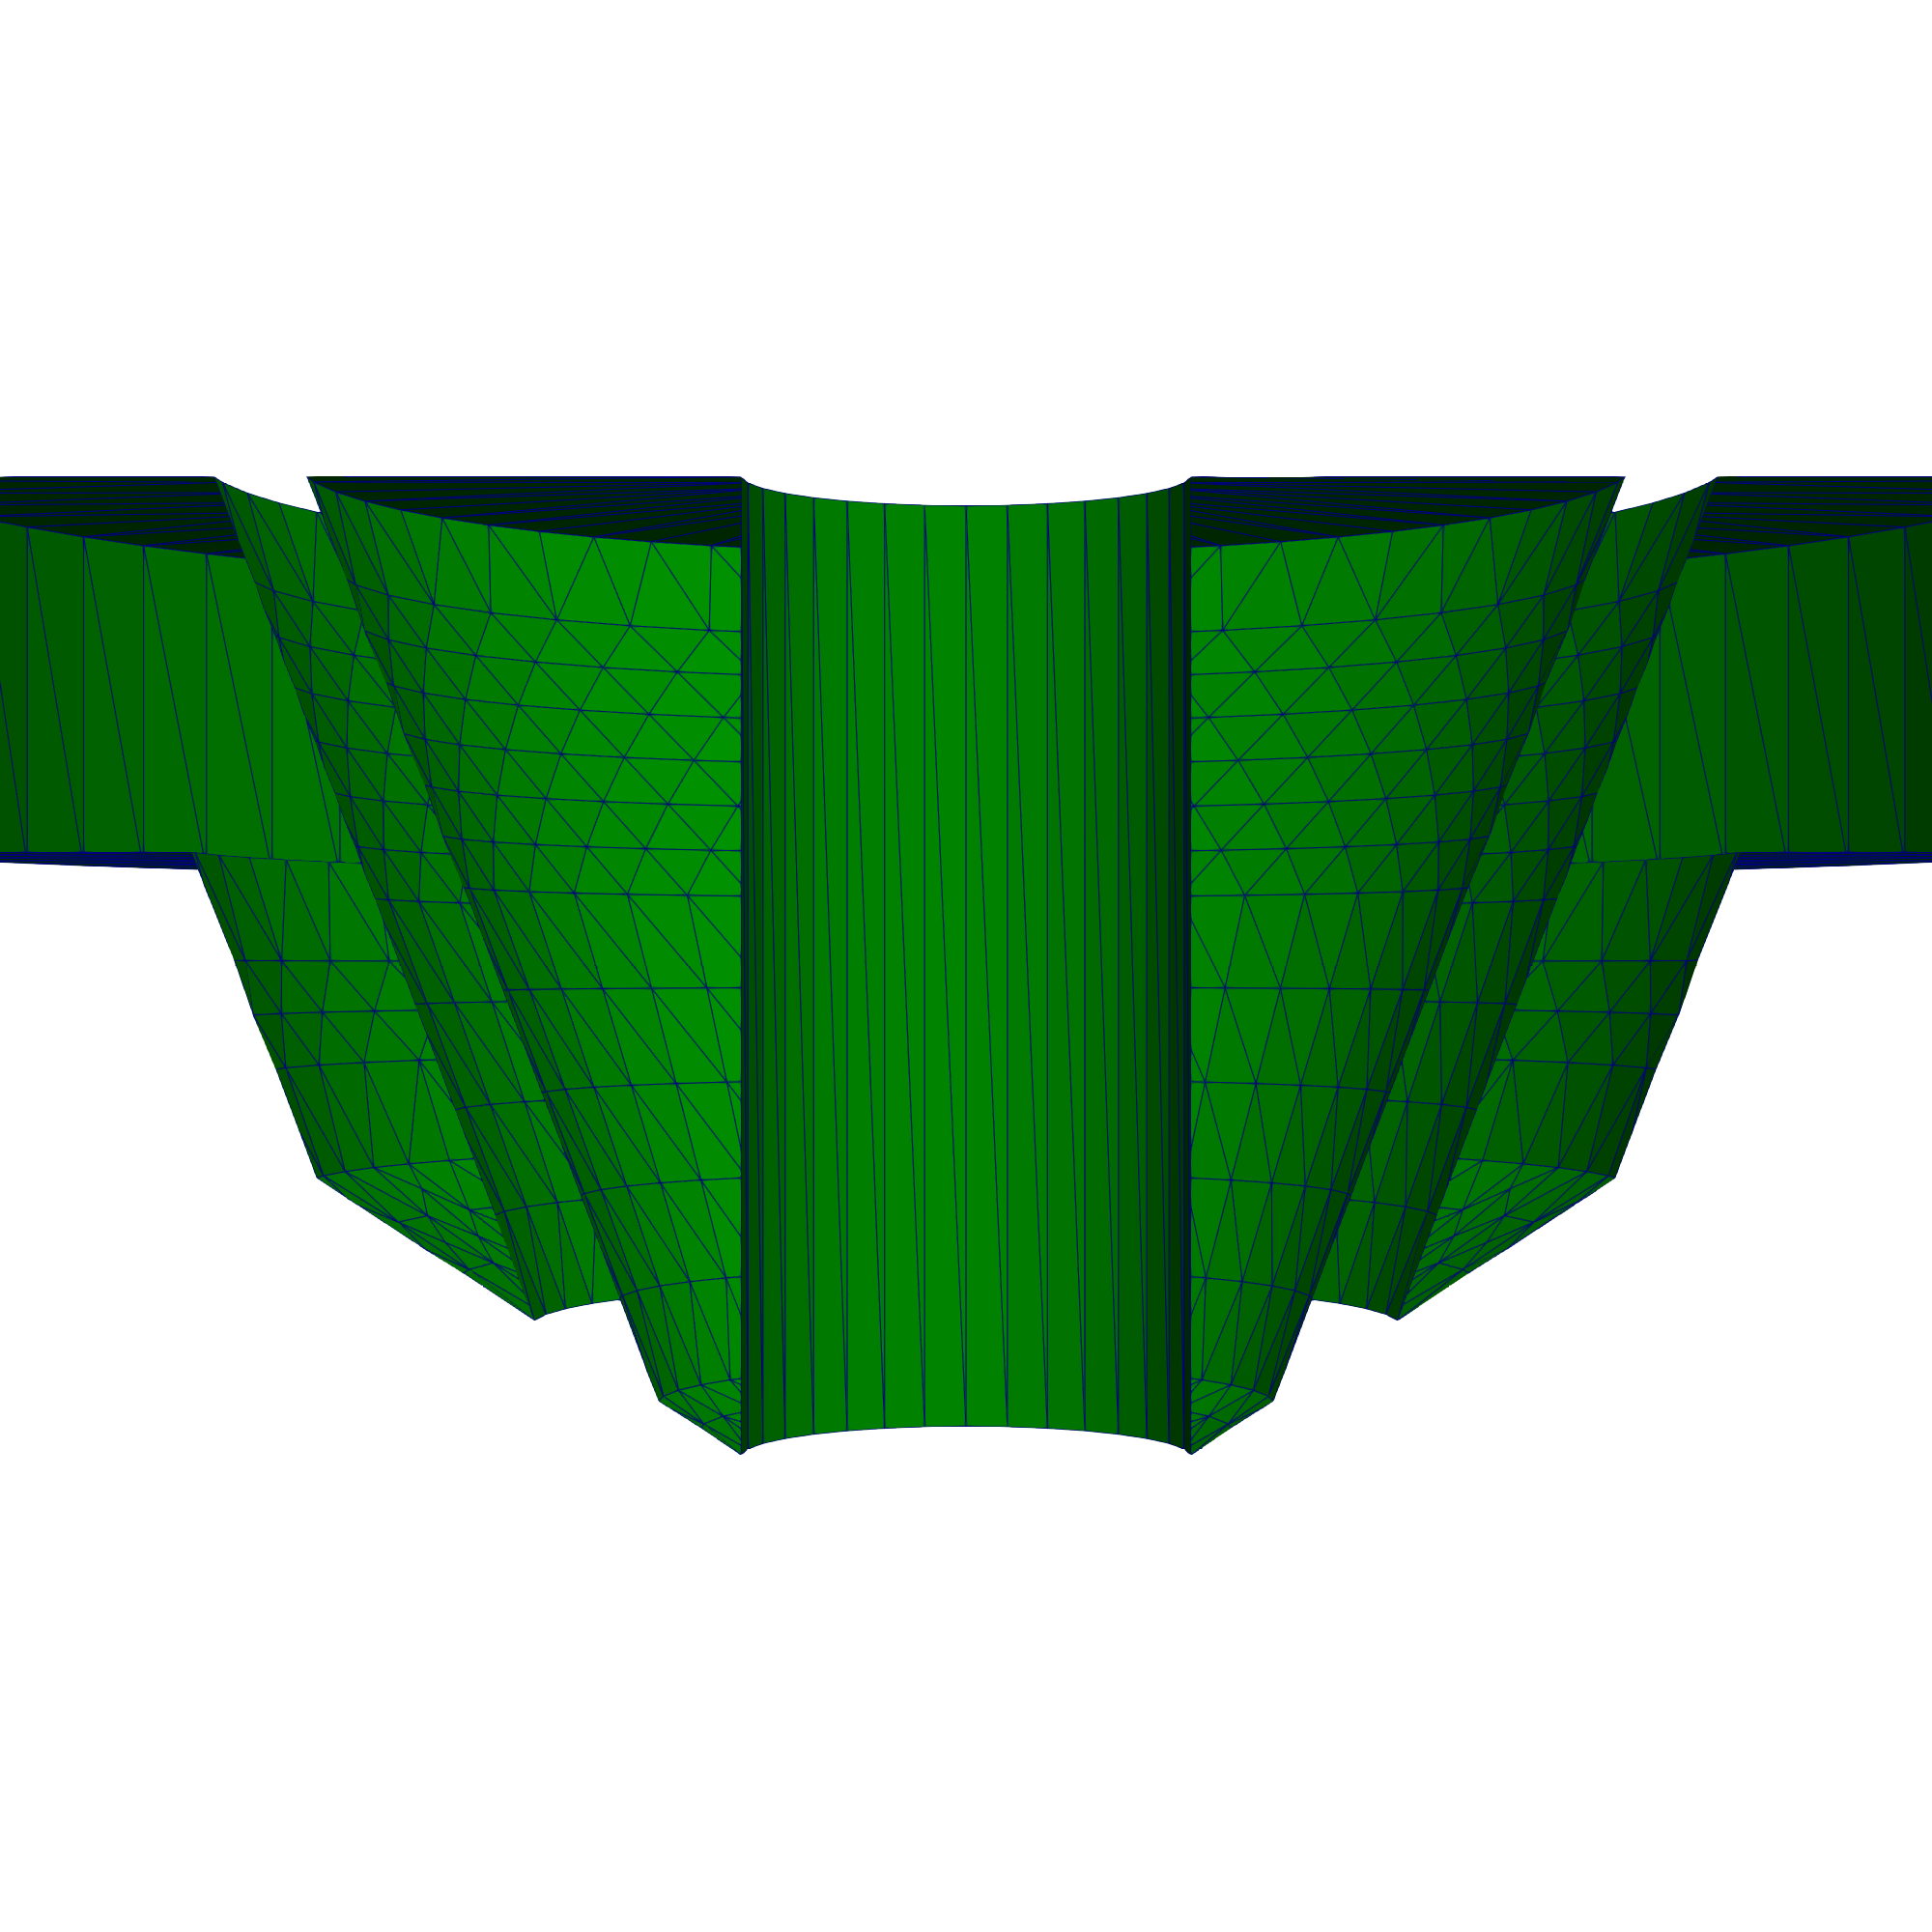
\includegraphics[width=\linewidth]{figure/screenshot_sezione_ugello.png}
    \caption{Ugello sezione laterale.}
\end{figure}

\begin{figure}[H]\label{dettaglio_ugello}
    \centering
    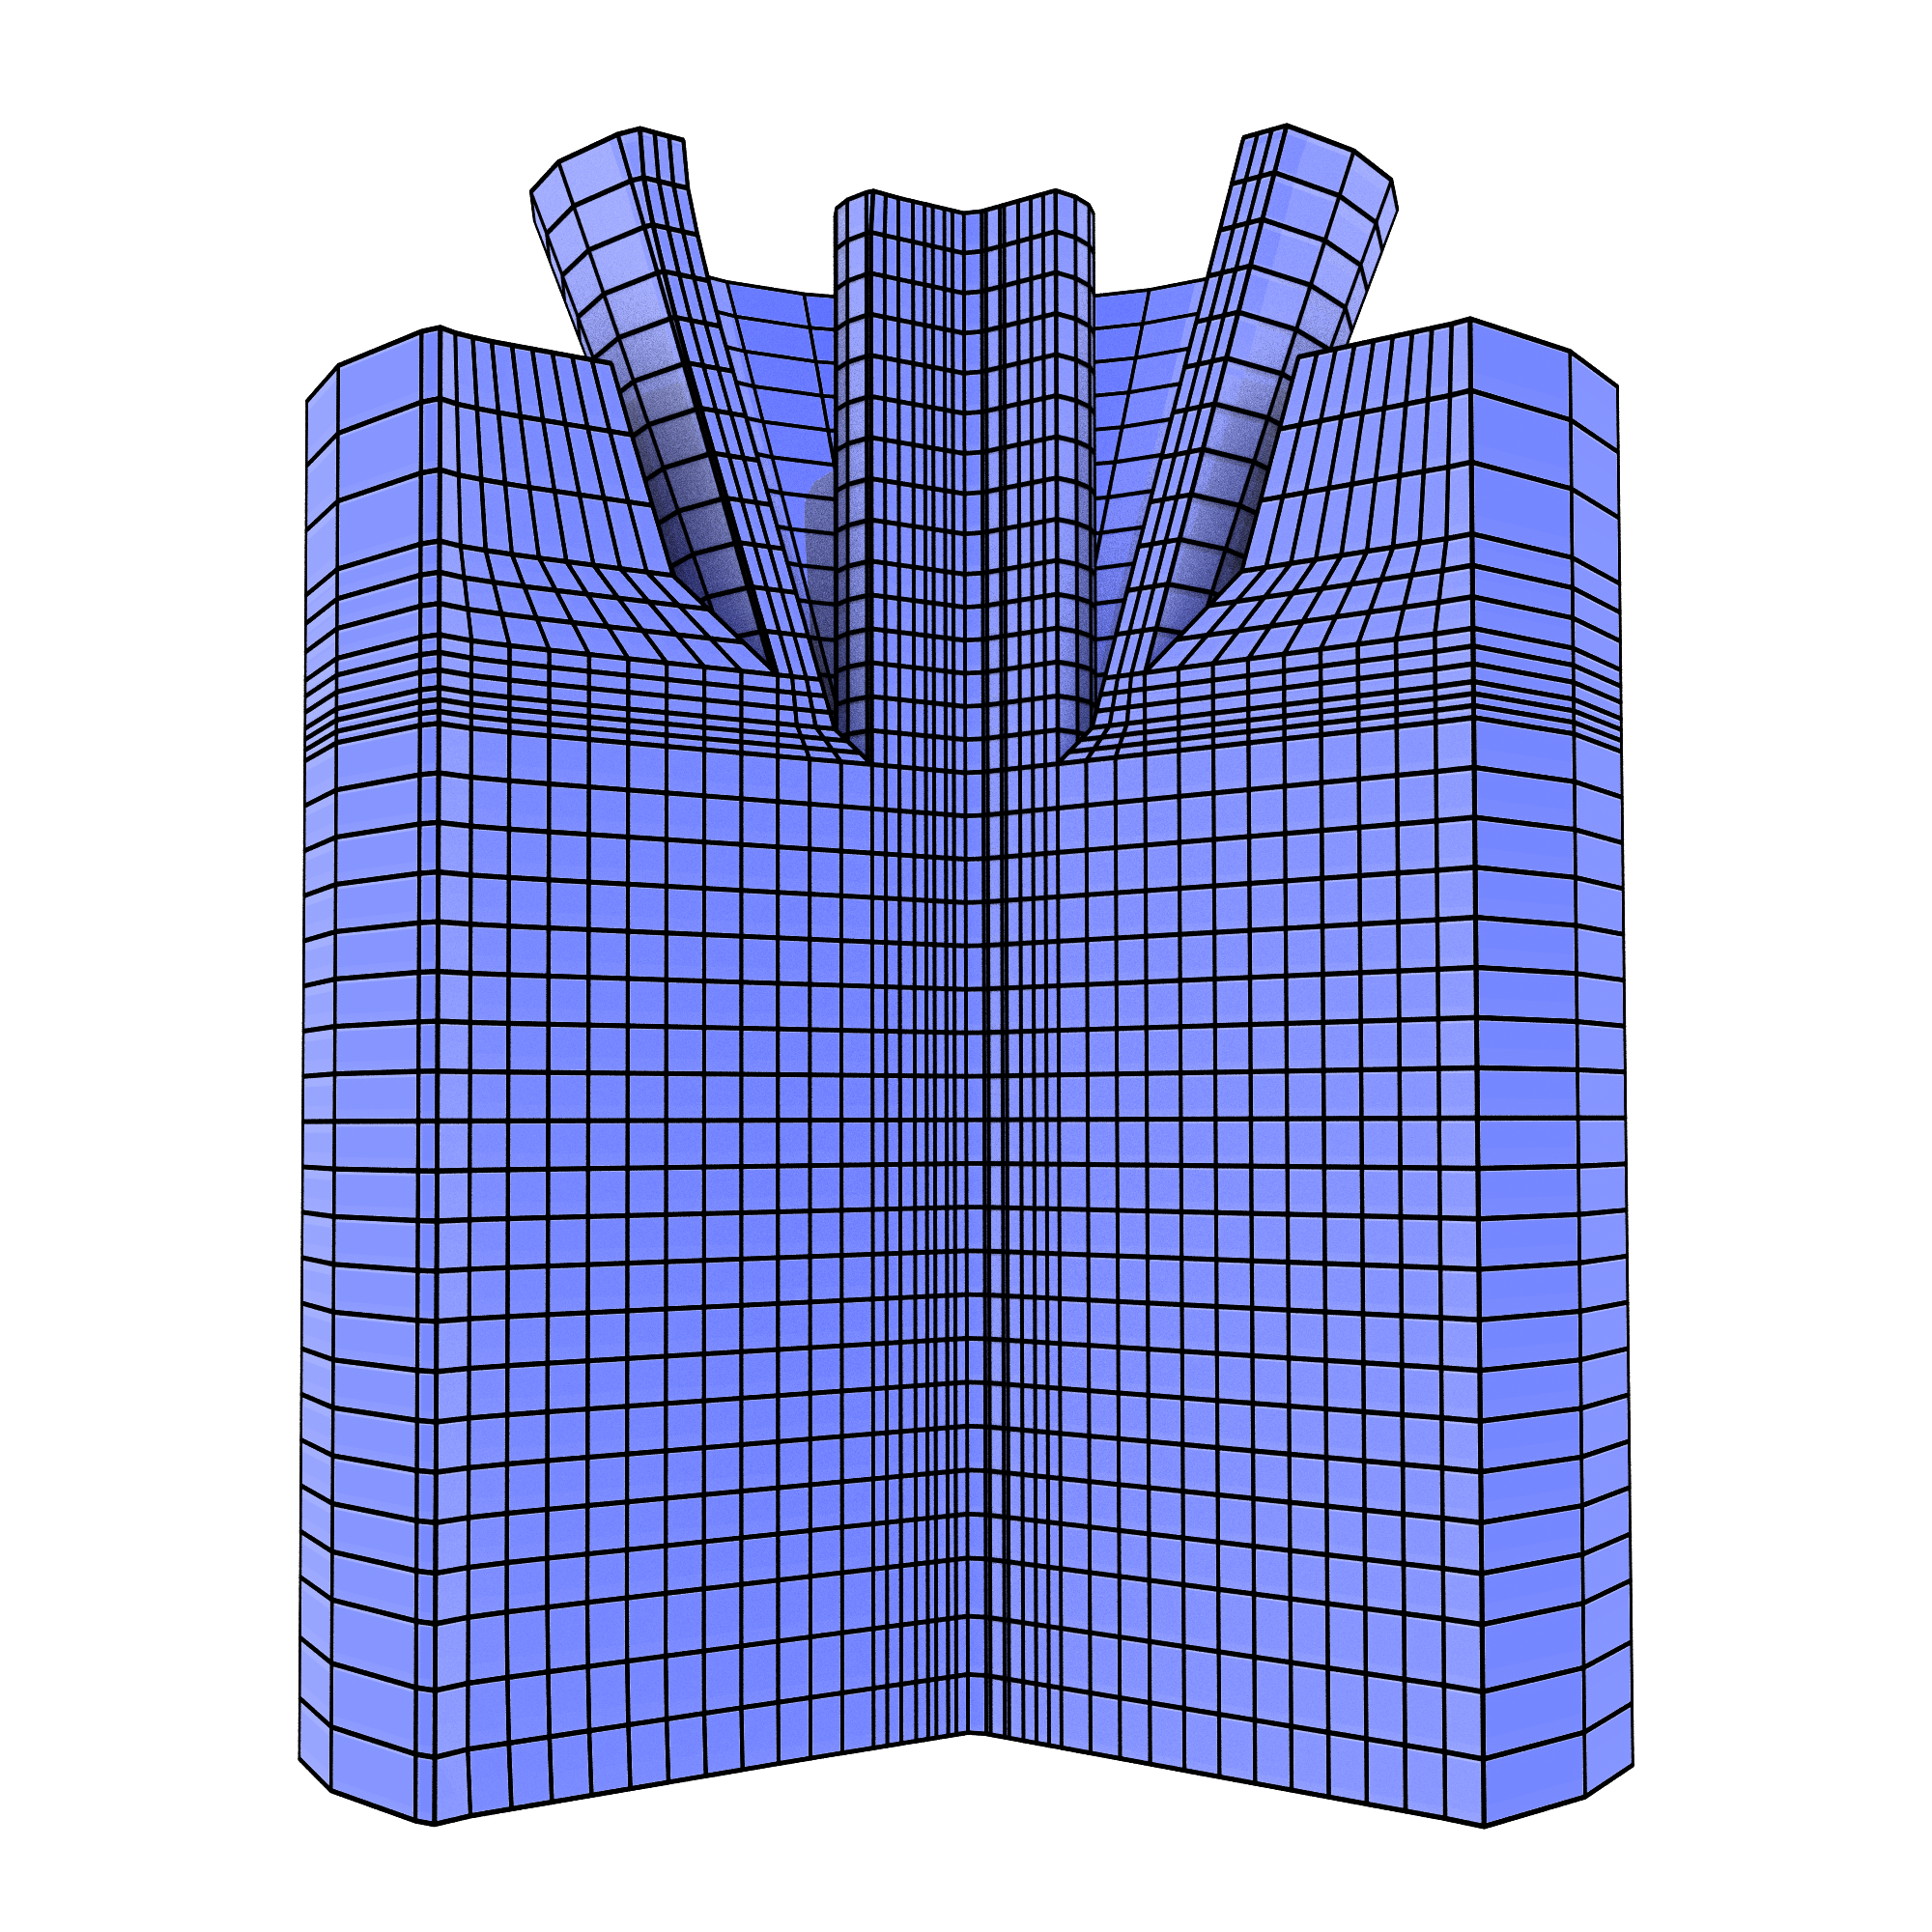
\includegraphics[width=\linewidth]{figure/presentazione_mesh.png}
    \caption{Mesh utilizzata per la simulazione.}
\end{figure}

\section{Fluido}
Analizzando l'immagine seguente notiamo una sezione dell'ugello in verde e il flusso di gas all'interno dello stesso in gradazioni di blu e rosso, in base alla velocità assunta.
Tralasciando gli errori di visualizzazione e compenetrazione dovuti a come Paraview visualizza gli oggetti sovrapposti, notiamo che il fluido viene accelerato nei condotti dell'ugello
e acquista velocità in fase di uscita. Questo comportamento è supportato dal fatto che la pressione è maggiore nella parte più alta dell'ugello.
\begin{figure}[H]\label{dettaglio_flusso}
    \centering
    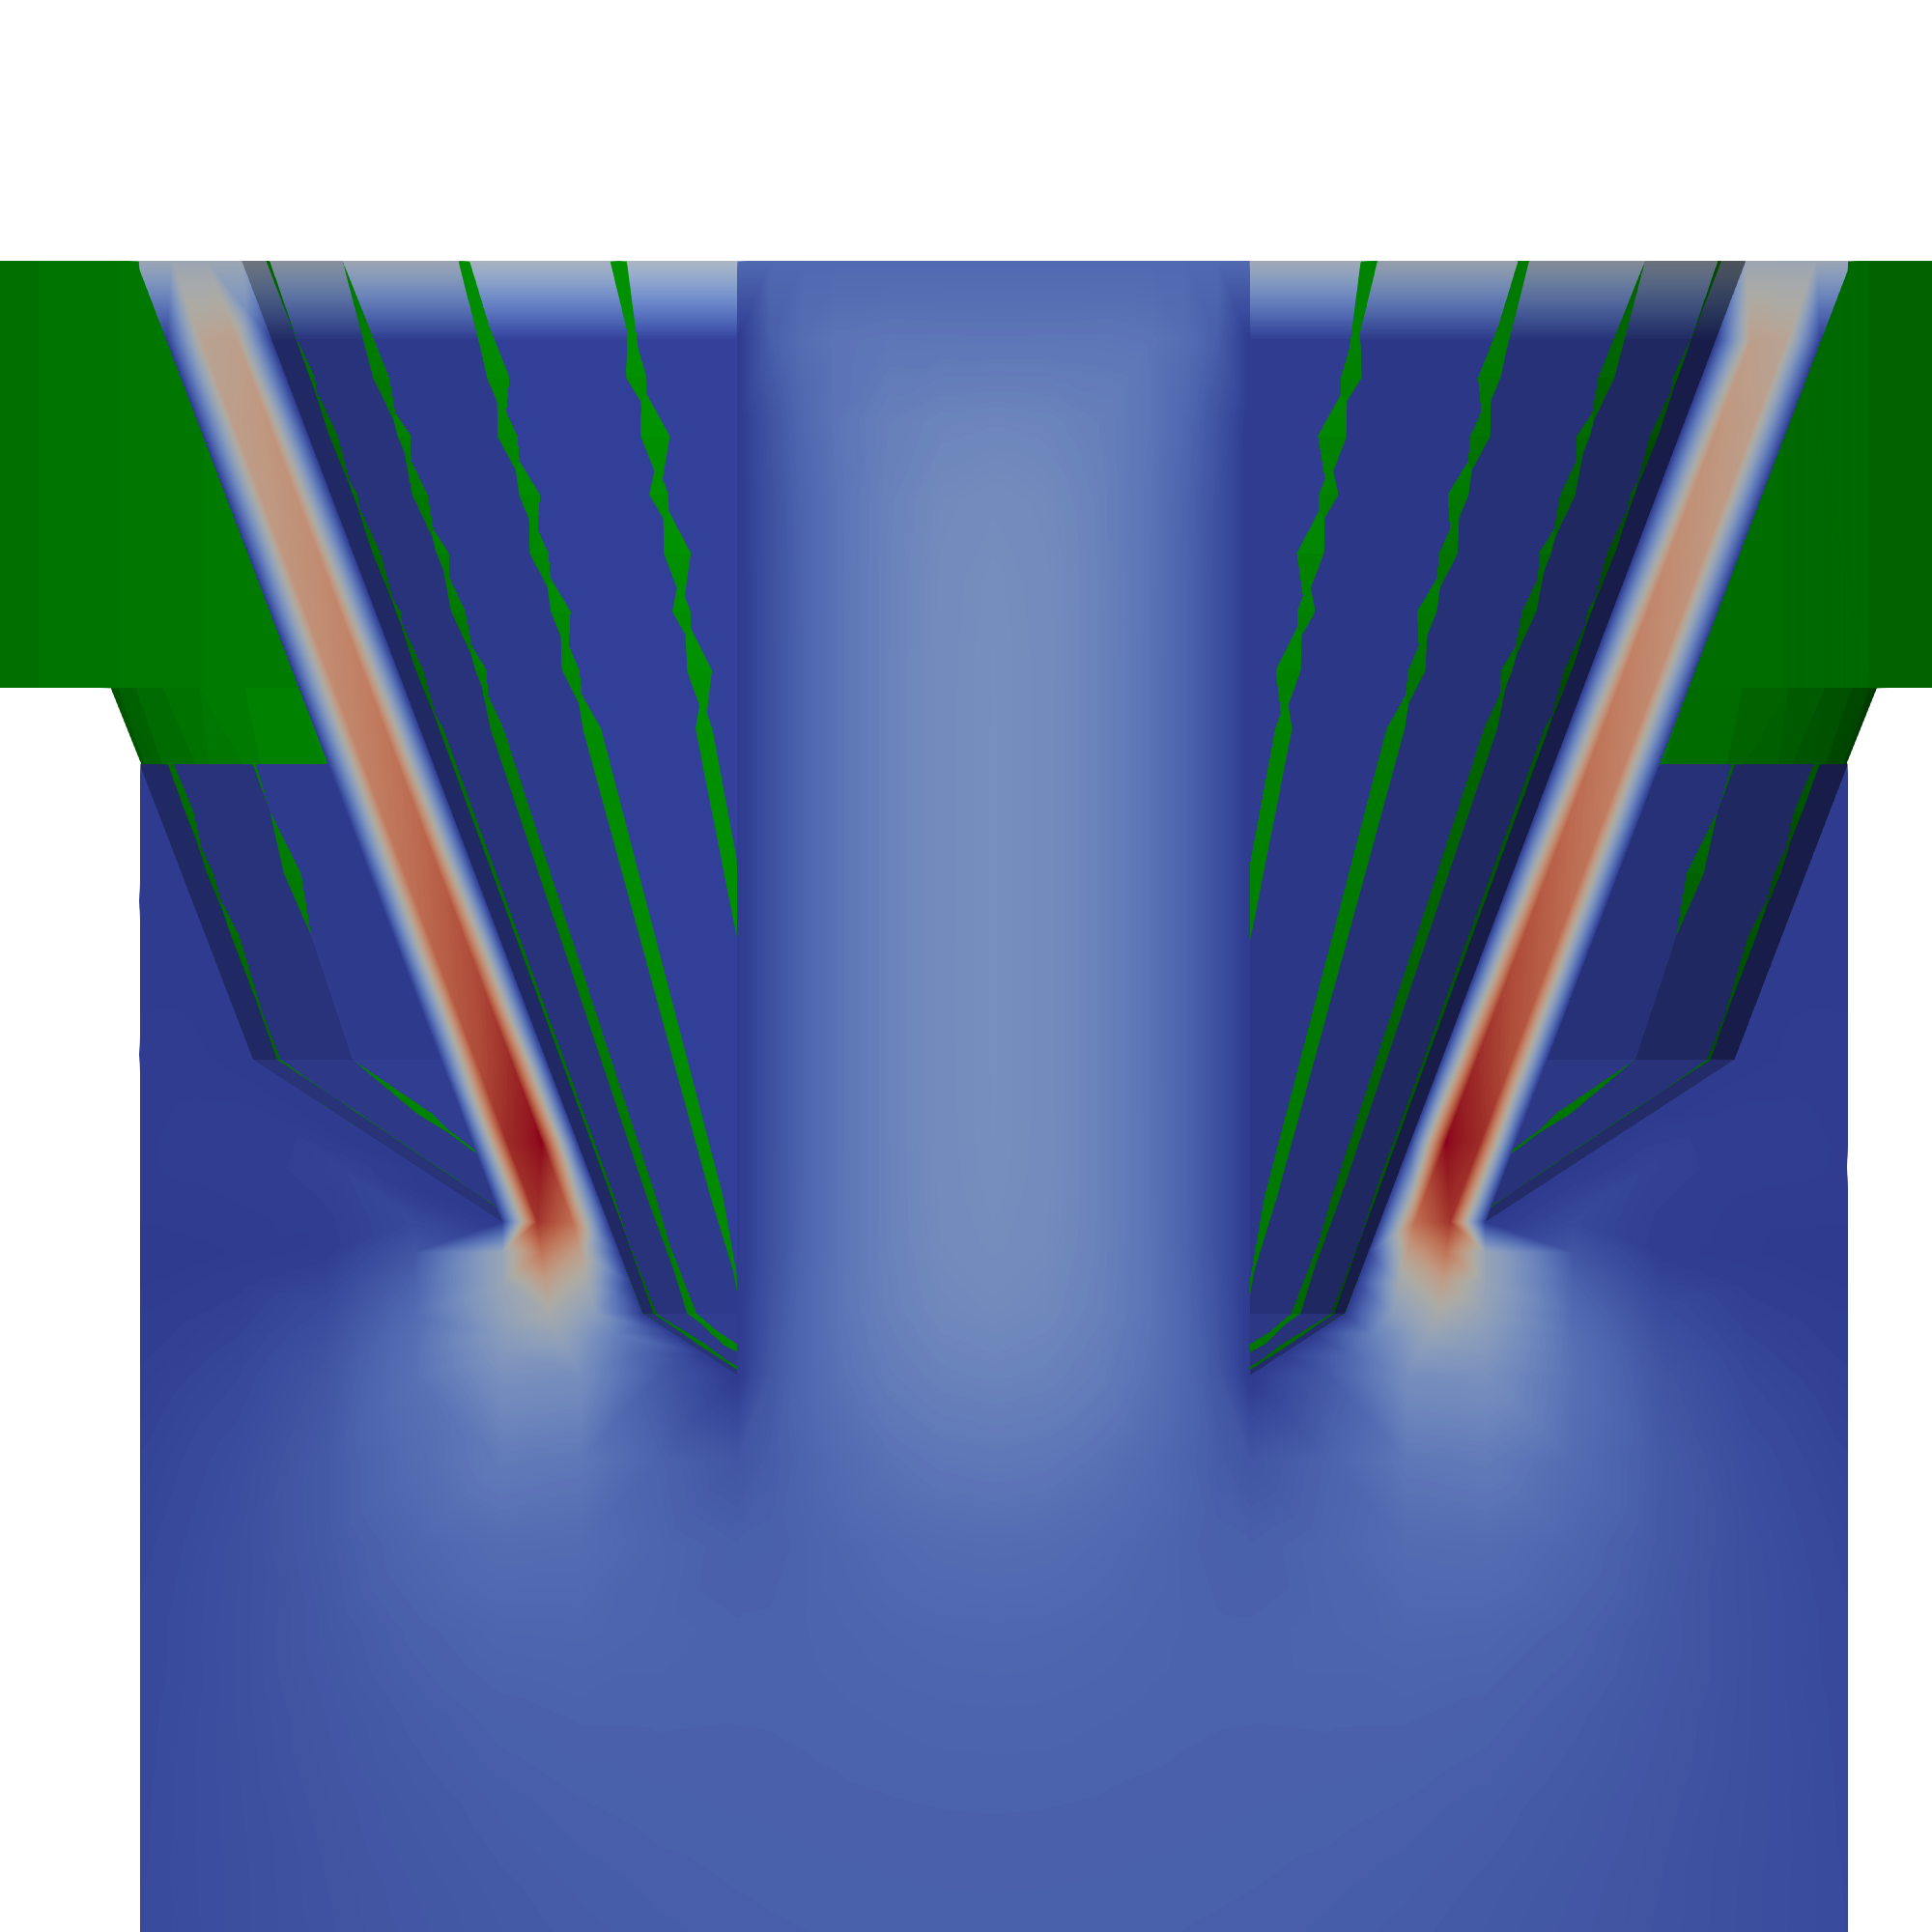
\includegraphics[width=\linewidth]{figure/screenshot_dettaglio_flussovel_ugello.png}
    \caption{Dettaglio flusso in entrata ugello, sezione laterale. Velocità fluido.}
\end{figure}
\begin{figure}[H]\label{dettaglio_flusso}
    \centering
    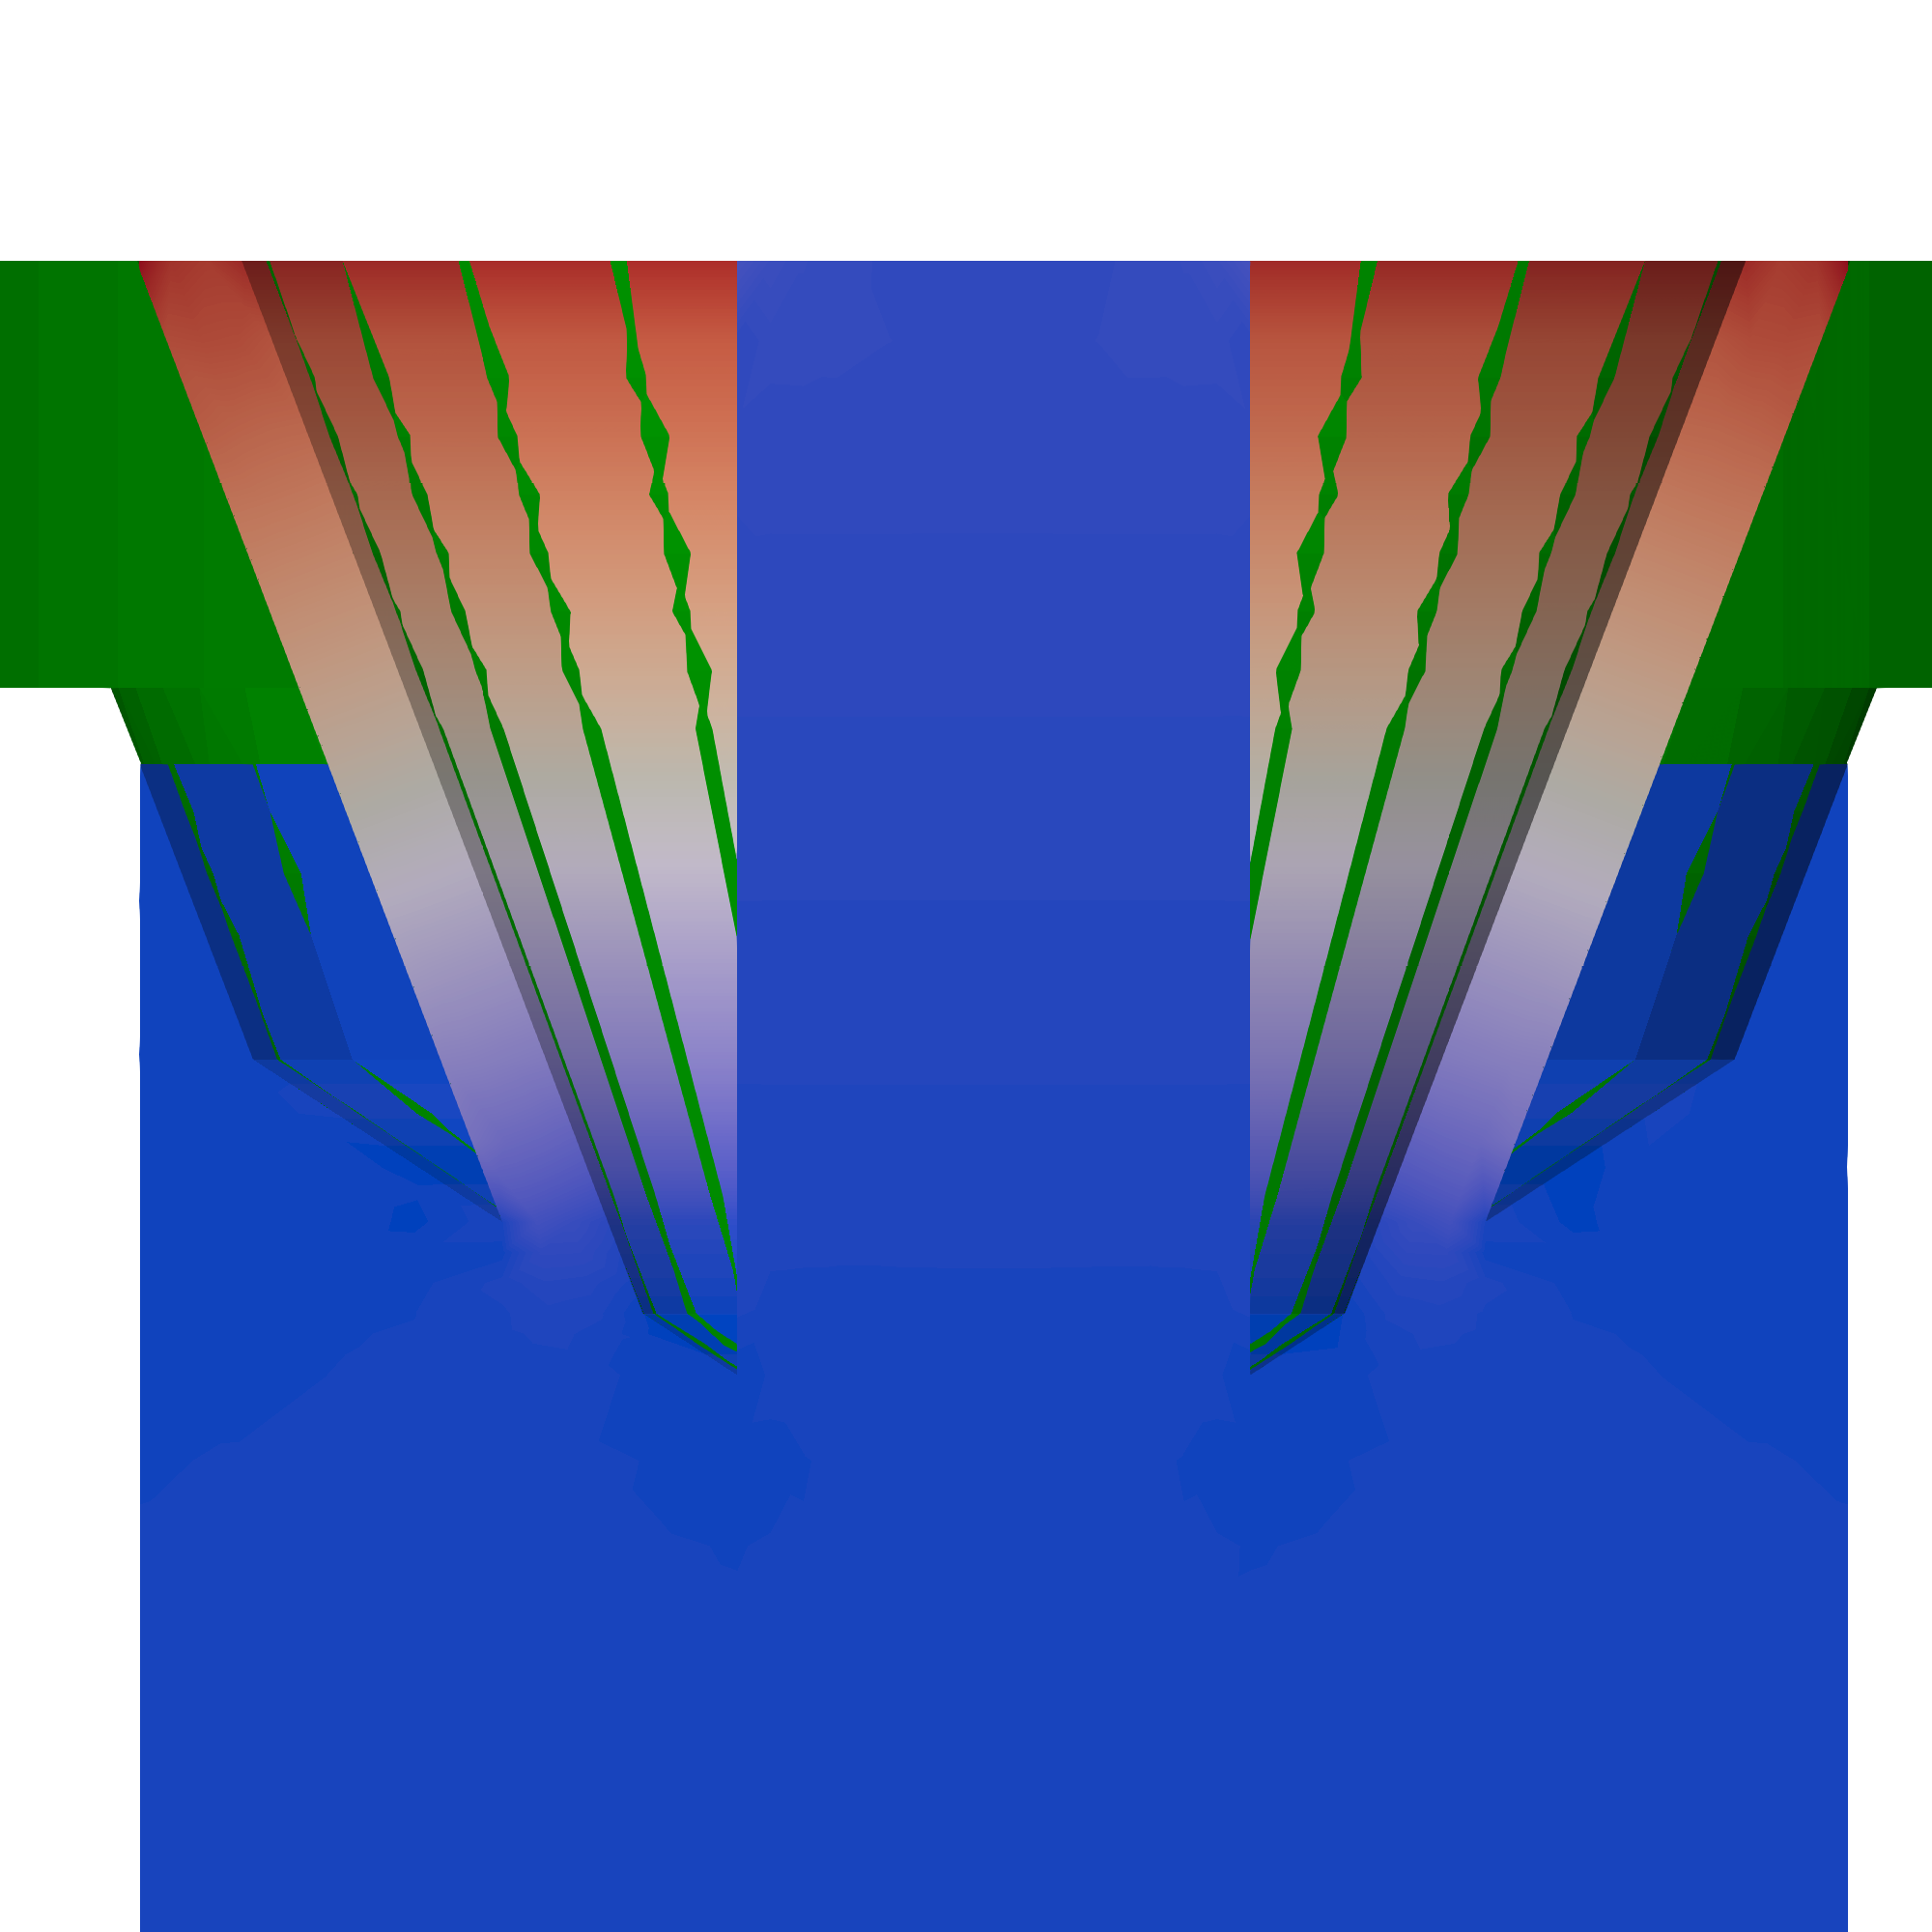
\includegraphics[width=\linewidth]{figure/screenshot_dettaglio_flussopres_ugello.png}
    \caption{Dettaglio flusso in entrata ugello, sezione laterale. Pressione fluido.}
\end{figure}
Per realizzare il gruppo di immagini precedente è stato importato il gruppo di file \texttt{VTK} prodotto dal solutore all'interno di Paraview. 
Una volta importato è stato applicato un filtro di tipo \texttt{Clip} che ci permette di sezionare la mesh rispetto a un'asse. 
In questo caso il clip è stato aggiunto in prossimità del centro lungo l'asse verticale. Il gradiente di velocità e pressione è stato impostato automaticamente 
da paraview in quanto nel file generato sono stati inclusi i rispettivi campi vettoriali (come visto nella sezione \ref*{5:output}). Infine come ultimo passaggio è stata 
attivata la vista ortografica in due dimensioni per eliminare distorsioni nel render.

\section{Laser}
Il laser viene simulato come un cilindro, che passa per il vertice del cono centrale, al cui interno si registra una temperatura più alta rispetto al resto del volume.
Nell'immagine sottostante è possibile notare come il fascio si propaga per tutto il volume e non intersechi l'ugello.
\begin{figure}[H]
    \centering
    
\includegraphics[width=\linewidth]{figure/screenshot_laser.png}
    \caption{Ugello con radiazione laser, sezione laterale.}
\end{figure}
Il procedimento per produrre quest'immagine è identico a quello precedente, con l'accortezza, però, di attivare il gradiente per il campo scalare relativo alla radiazione laser.

\section{Particelle}
Analizziamo ora in maniera dettagliata la generazione delle particelle e la loro simulazione.
Nella seguente immagine è possibile valutare, tramite una vista dall'alto della soluzione, l'anello di particelle che si genera nella fase iniziale della simulazione.
Per importare il file \texttt{CSV} all'interno di Paraview è stato utilizzato un filtro chiamato "TableToPoints", che, dato in input proprio un file \texttt{CSV}, permette di mappare 
ogni riga del file a punti nello spazio tridimensionale.
Per rendere più visibili le particelle è stato omesso il fluido e l'ugello da questi render.
\begin{figure}[H]
    \centering
    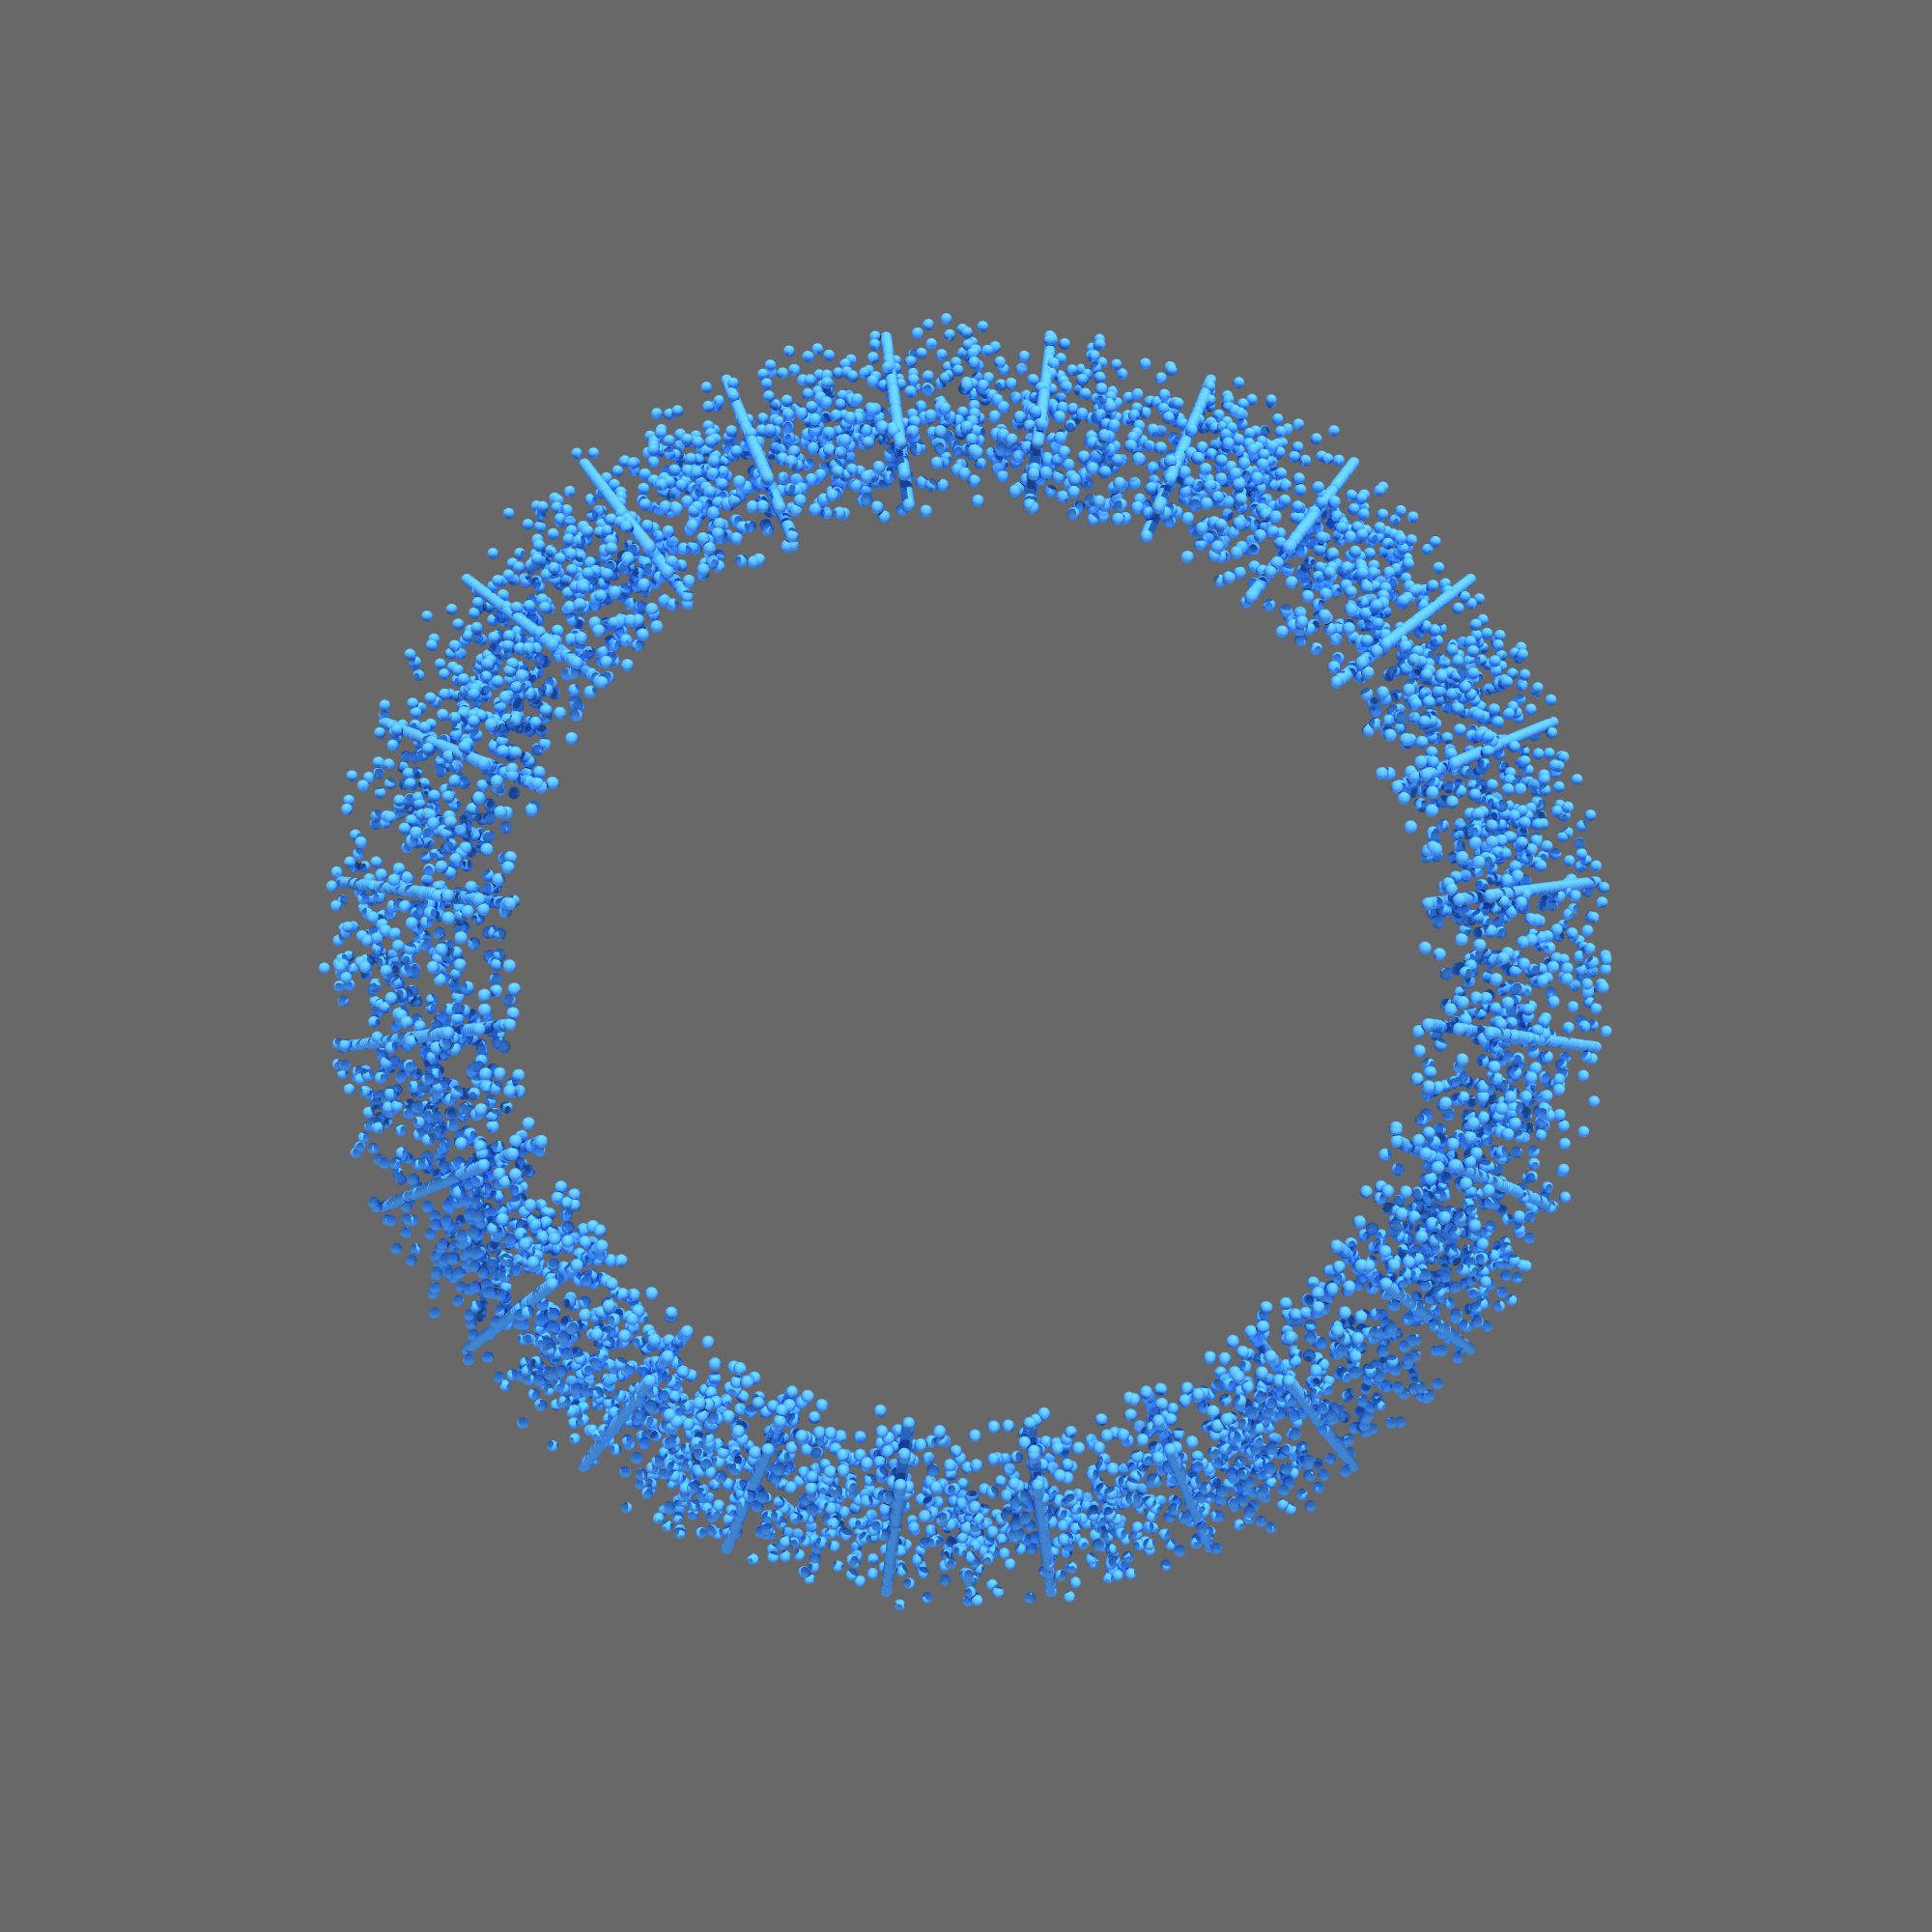
\includegraphics[width=\linewidth]{figure/screenshot_dettaglio_particelle_alto.png}
    \caption{Anello di particelle in entrata, vista dall'alto.}
\end{figure}
Come accennato in precedenza (\ref*{5:particelle}) le particelle possiedono un campo scalare che rappresenta la temperatura. Questo campo è univoco per particella e ci permette di applicare un
gradiente basato su di esso all'interno di Paraview. Intuibilmente il colore blu rappresenta particelle fredde, quello rosso calde.
\begin{figure}[H]
    \centering
    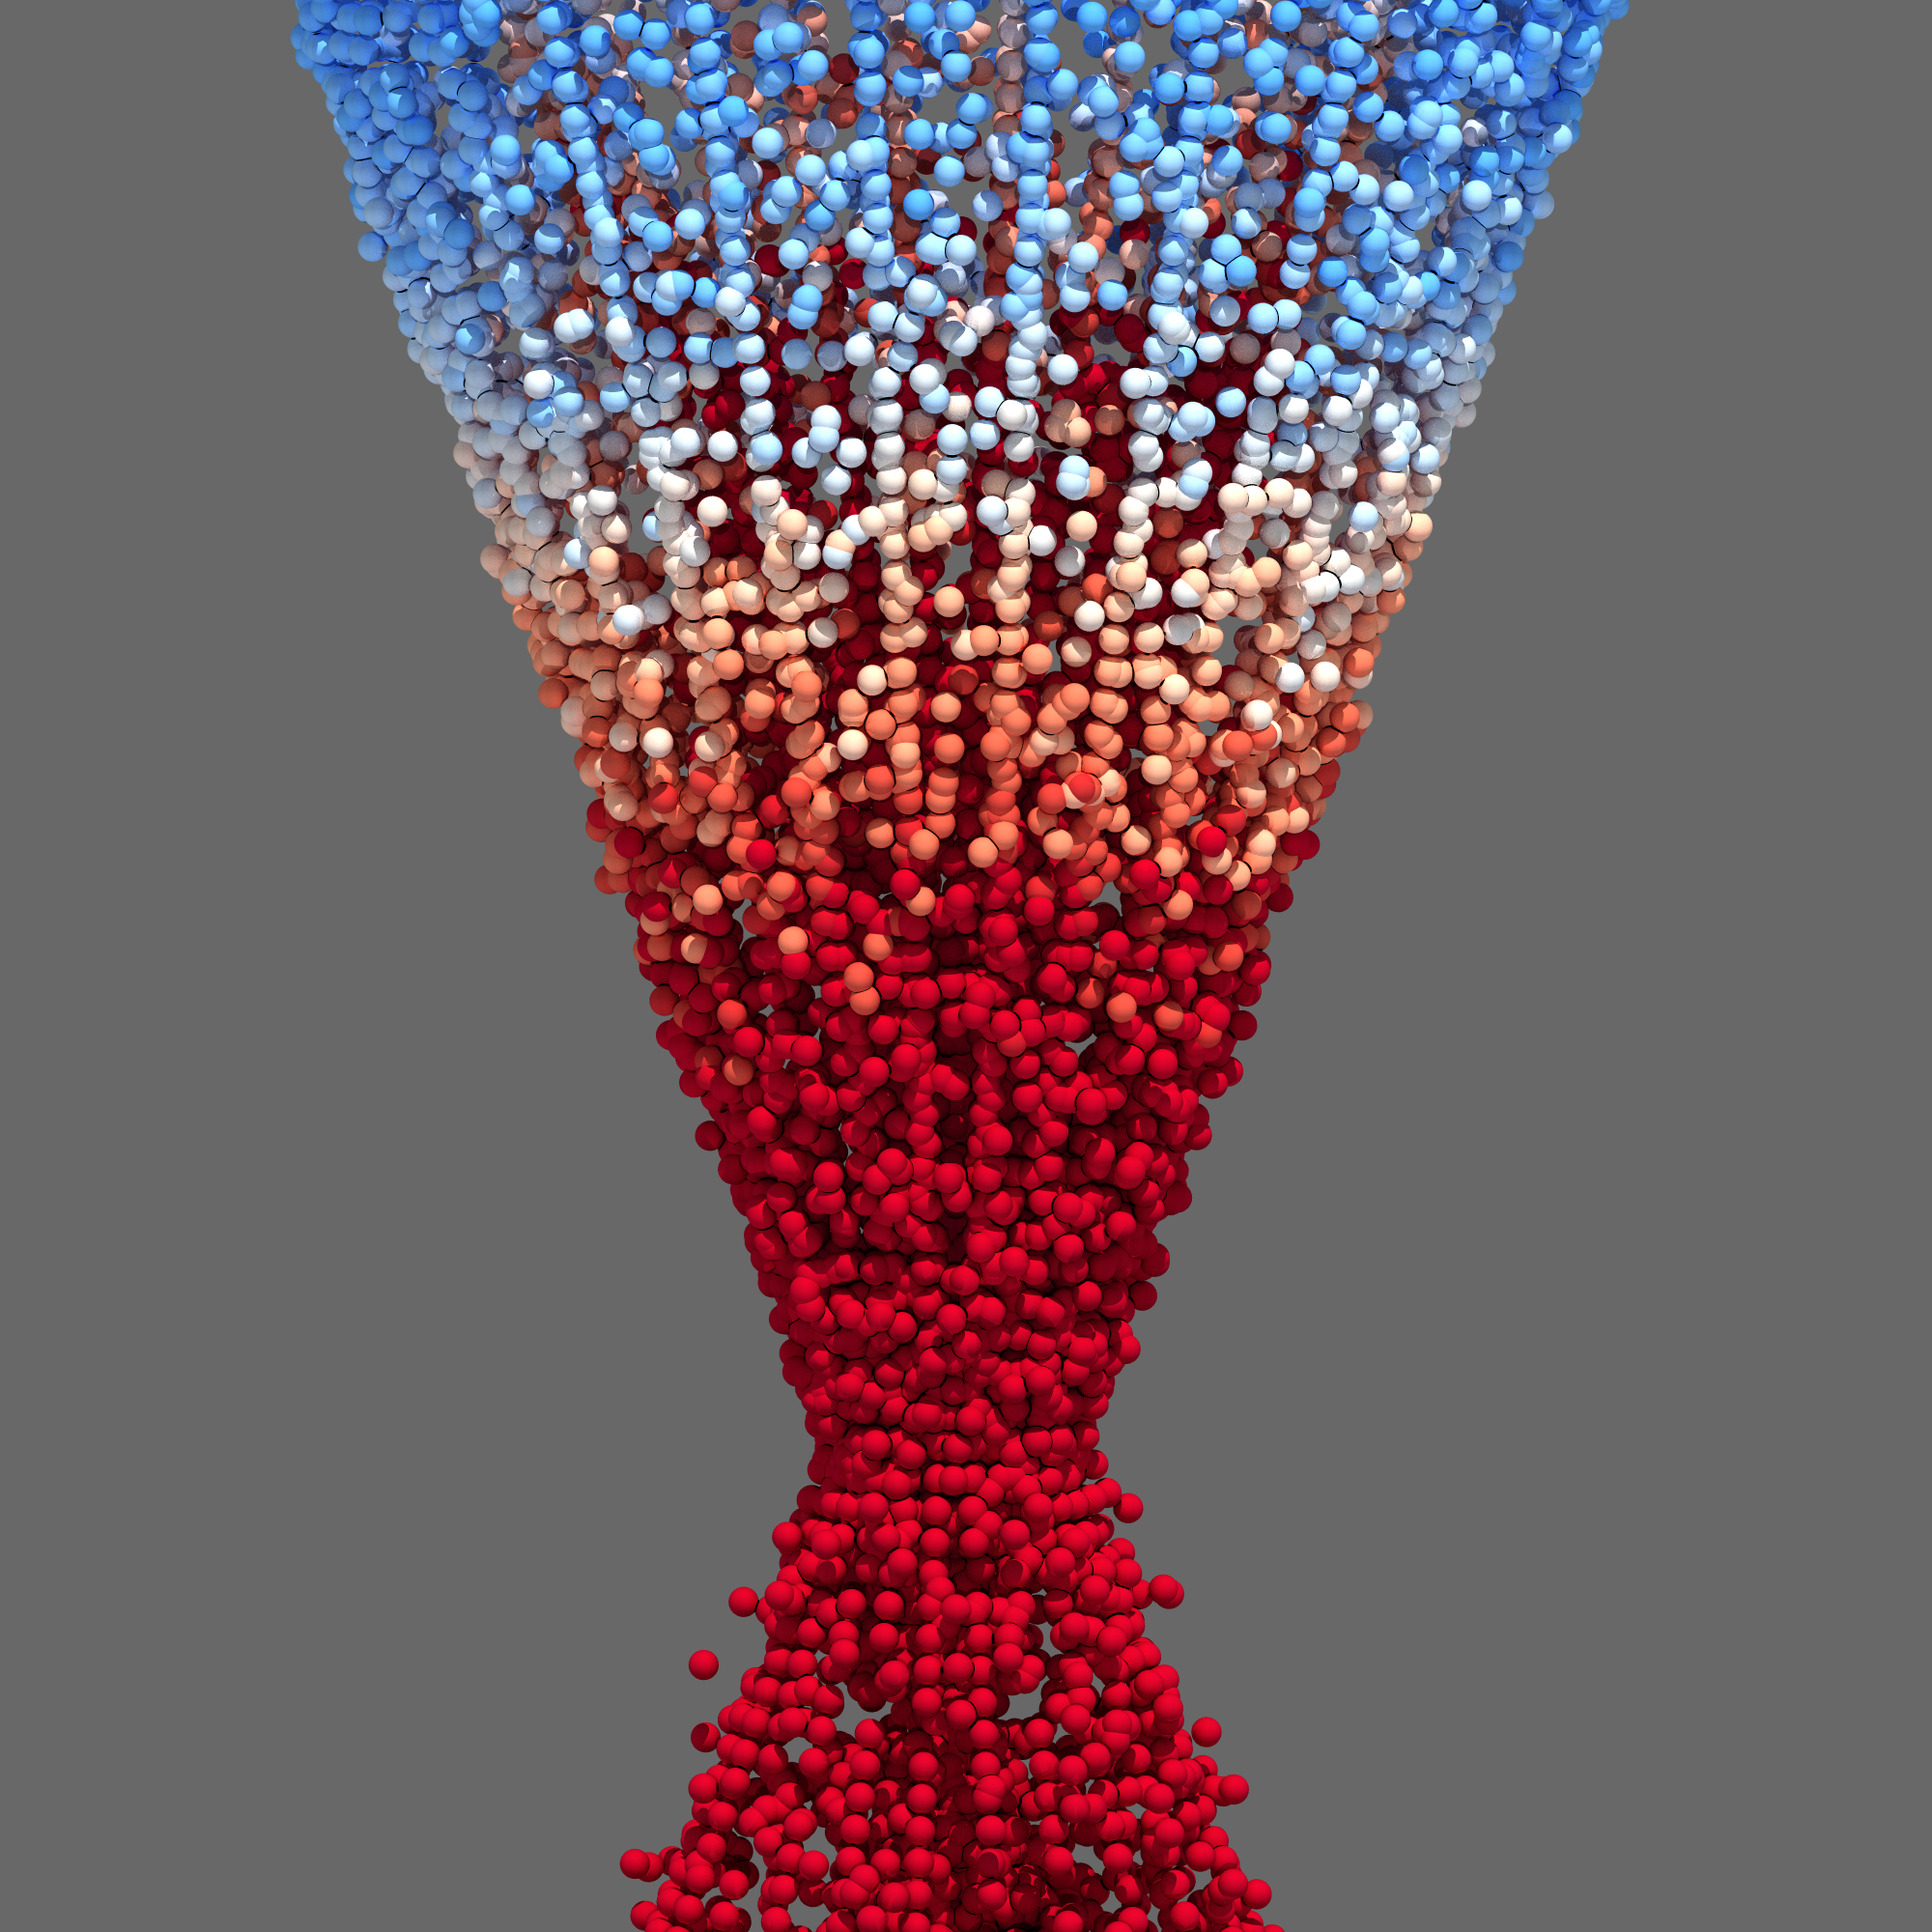
\includegraphics[width=\linewidth]{figure/screenshot_dettaglio_particelle.png}
    \caption{Particelle con colorazione basata su valori temperatura, vista laterale.}
\end{figure}
Notare come le particelle cambino temperatura proprio in corrispondenza del fascio laser.
\begin{figure}[H]
    \centering
    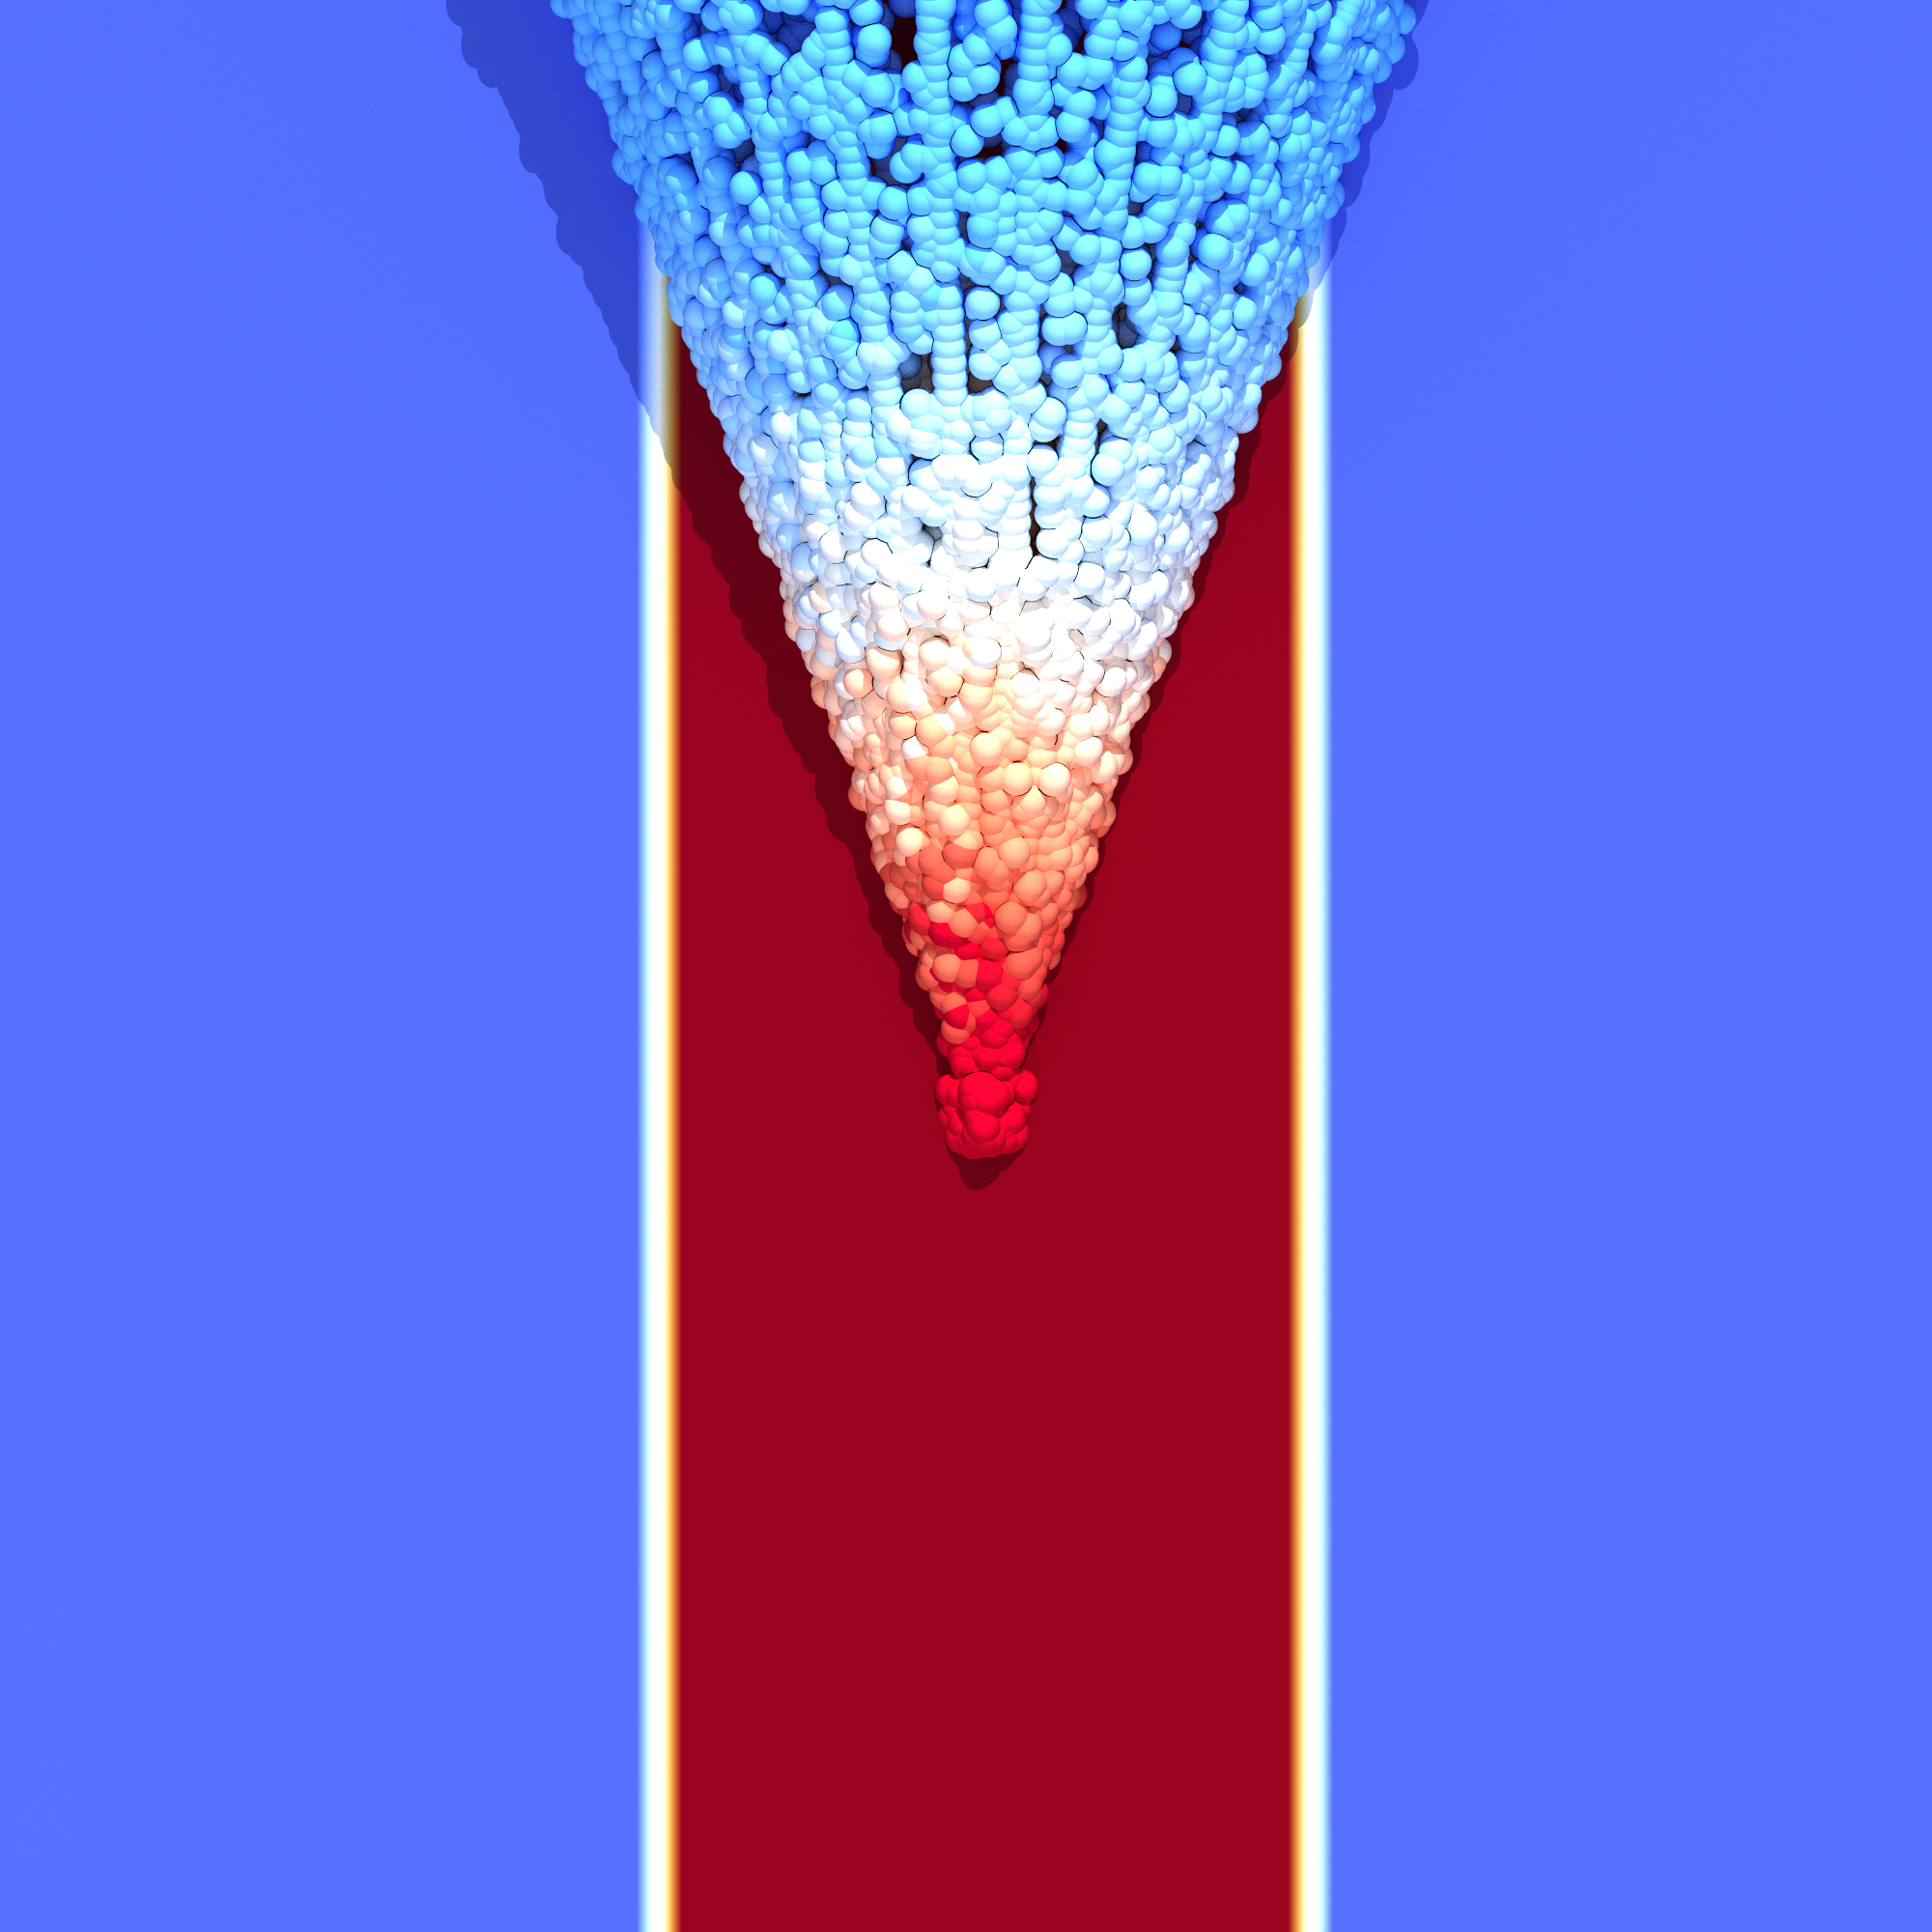
\includegraphics[width=\linewidth]{figure/screenshot_dettaglio_particelle_laser.png}
    \caption{Dettaglio particelle riscaldate da laser,sezione laterale.}
\end{figure}
Nei seguenti render è possibile vedere una sezione della completa simulazione, con ugello, velocità del flusso e particelle.
\begin{figure}[H]
    \centering
    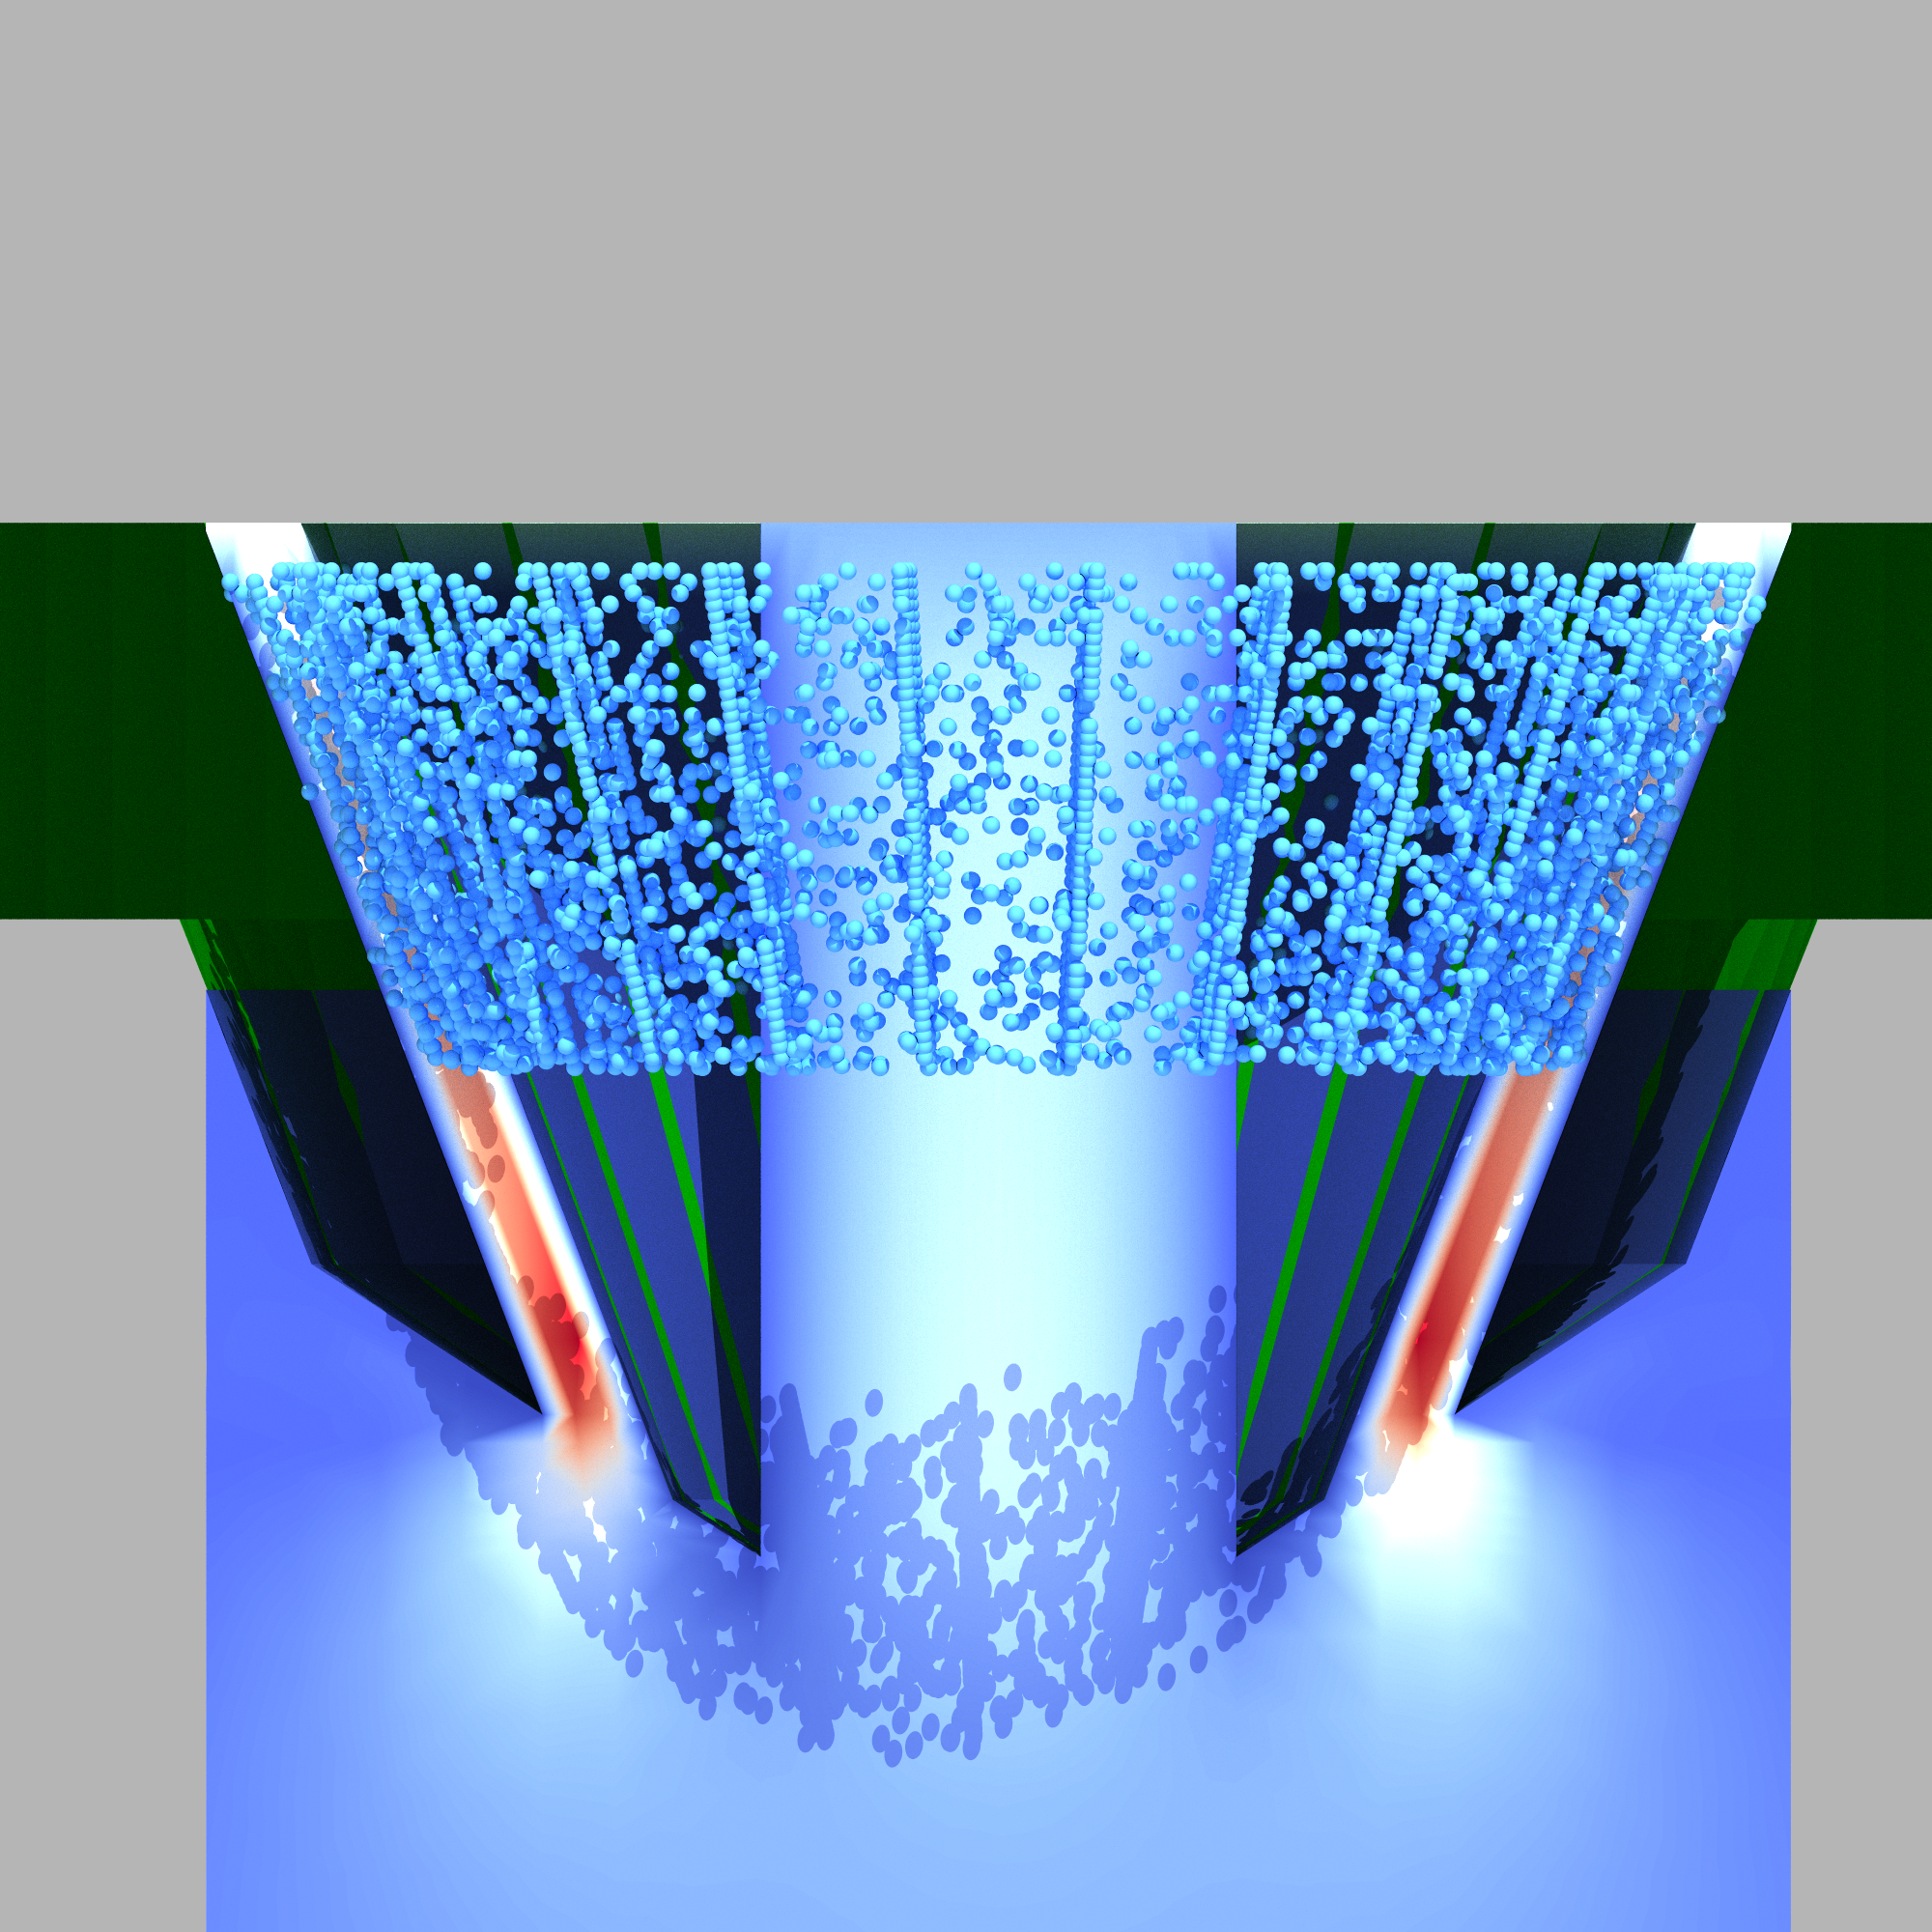
\includegraphics[width=\linewidth]{figure/screenshot_dettaglio_particelle_fluido.png}
    \caption{Dettaglio punto di entrata particelle con ugello e flusso, sezione laterale.}
\end{figure}
\begin{figure}[H]
    \centering
    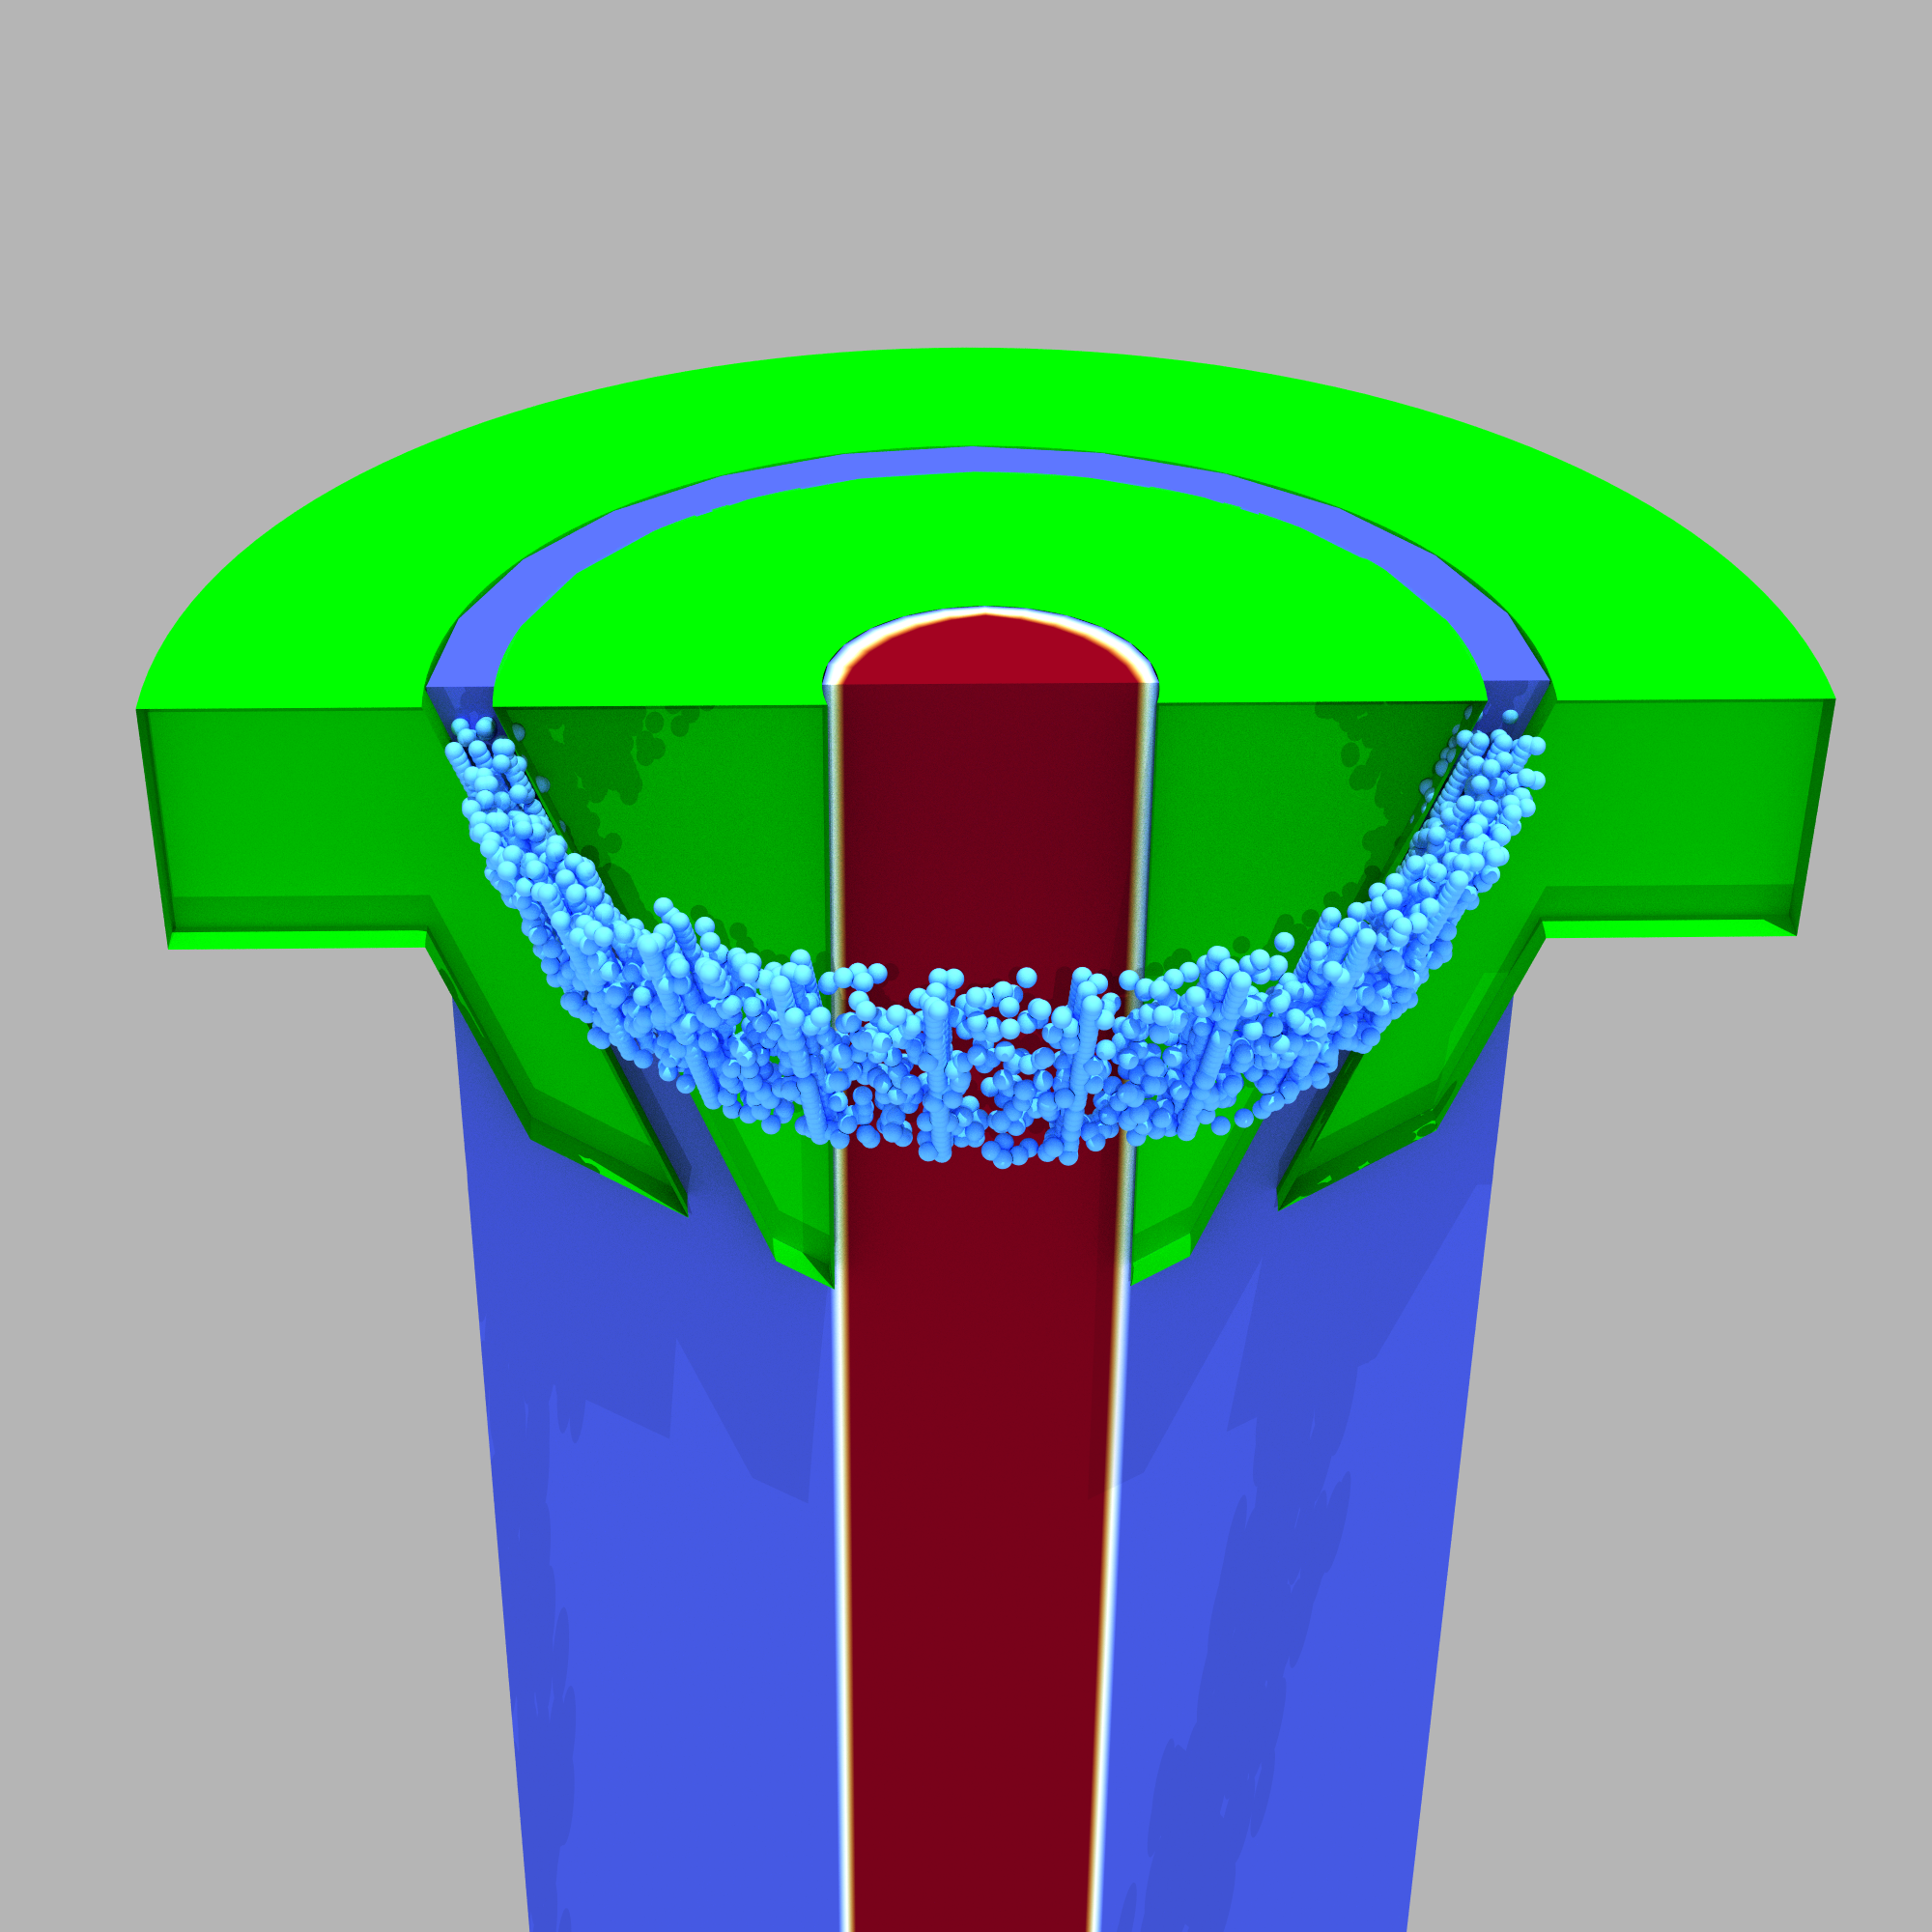
\includegraphics[width=\linewidth]{figure/screenshot_dettaglio_all_ugello.png}
    \caption{Dettaglio punto di entrata particelle con ugello e flusso, sezione laterale.}
\end{figure}